

\chapter{Linear Functions}

\section*{Introduction}

        In this Chapter, we will introduce the notion of a \textbf{linear function}.  Linear functions are used to model a variety of situations, such as the the revenue generated by selling a product, conversion between units of measurement such as Fahrenheit to Celsius, distance traveled by an entity moving at a constant velocity, demand of a product relative to price and many more.  It is also a good introduction to the theory of functions more generally.


\section{What is a Linear Function?}

A linear function is a function whose inputs and outputs are real numbers, and \textit{the change in output per unit change increase in input is always the same.}  A linear function may always increase, or decrease, or stay the same, but the rate at which it does so will never change.

\begin{example}
Consider a function who takes on the following values:

$$\begin{array}{|c||c|c|c|c|c|}
\hline
x & 1&2&3&4&10\\
\hline
f(x)&10&12&14&16&28\\
\hline
\end{array}
$$

\textbf{Question:} Does this function appear linear?\\

\textbf{Solution:} It certainly takes on the semblance of linearity, if we observe the change from $x=1$ to $x=2$, the change in $f(x)$ or $\Delta f(x)=12-10=2$. 

 When we go from $x=2$ to $x=3$, we again saw that $\Delta f(x)=14-12=2$, and so forth.  
 
 Even when we go from $x=4$ to $x=10$, we say that $\Delta f(x)=28-16=12$, but that was over a change of $\Delta x=10-4=6$.  This is still a change of $12/6=2$ per unit of $x$.  So assuming nothing wild happens between the listed values, this function does seem linear.

Graphically we can visualize this:

$$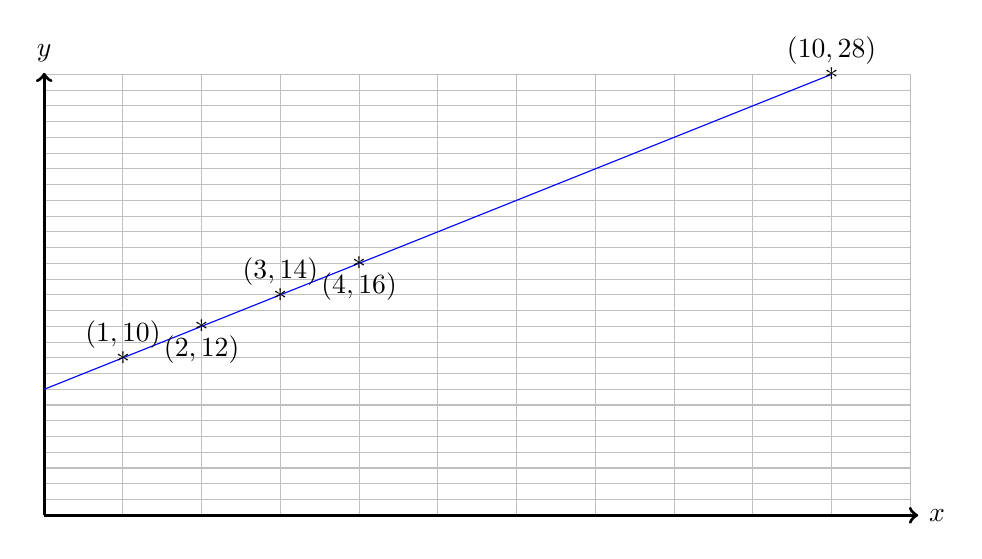
\begin{tikzpicture}[yscale=.2][domain=-0:11]
    \draw[gray!50, thin, step=1] (0,0) grid (11,28);
    \draw[very thick,->] (0,0) -- (11.1,0) node[right] {$x$};
    \draw[very thick,->] (0,0) -- (0,28.1) node[above] {$y$};

%    \foreach \x in {0,...,11} \draw (\x,0.05) -- (\x,-0.05) node[below] {\tiny\x};
%    \foreach \y in {0,...,28} \draw (-0.05,\y) -- (0.05,\y) node[right] {\tiny\y};


  \draw[scale=1,domain=0:10,smooth,variable=\x,blue] plot ({\x},{2*\x+8});

\node at (1,10){$*$};
\draw (1,10) --node[above]{$(1,10)$}(1,10);

\node at (2,12){$*$};
\draw (2,12) --node[below]{$(2,12)$}(2,12);

\node at (3,14){$*$};
\draw (3,14) --node[above]{$(3,14)$}(3,14);

\node at (4,16){$*$};
\draw (4,16) --node[below]{$(4,16)$}(4,16);

\node at (10,28){$*$};
\draw (10,28) --node[above]{$(10,28)$}(10,28);




\end{tikzpicture}$$ % of mbox

An interactive version of this graph may be found here: \url{https://www.desmos.com/calculator/9hocfhhs1m}.


\end{example}


It always helps to illustrate a concept with a \textbf{non}-example.

\begin{example}
Consider a function who takes on the following values:

$$\begin{array}{|c||c|c|c|c|c|}
\hline
x & -2&-1&0&1&2\\
\hline
f(x)&4&1&0&1&4\\
\hline
\end{array}
$$

\textbf{Question:} Does this function appear linear?\\

\textbf{Solution:}If we observe the change from $x=-2$ to $x=-1$, the change in $f(x)$ or $\Delta f(x)=1-4=-3$. 

 However, when we go from $x=-1$ to $x=0$, we see that $\Delta f(x)=0-1=-1$.  Similarly,   when we go from $x=0$ to $x=1$, we see that $\Delta f(x)=1-0=1$, and when we go from $x=1$ to $x=2$, we see that $\Delta f(x)=4-1=3$.
 
 Thus, this function goes from decreasing, to increasing, and the rate at which it does so changes, thus this function is \textbf{not} a linear function.


Graphically we can visualize this:

$$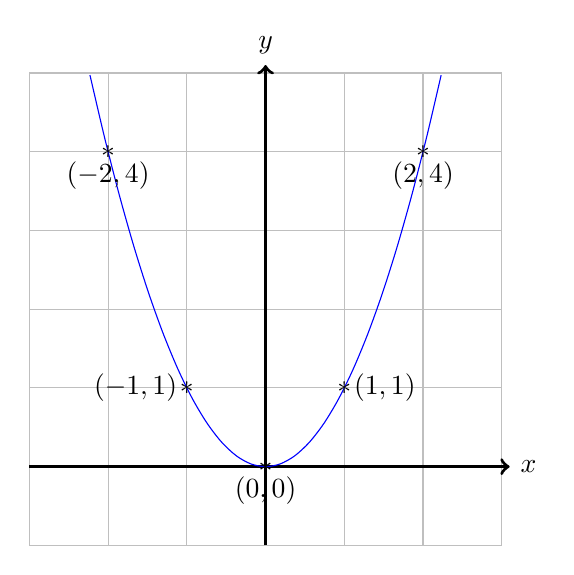
\begin{tikzpicture}[scale=1][domain=-0:11]
    \draw[gray!50, thin, step=1] (-3,-1) grid (3,5);
    \draw[very thick,->] (-3,0) -- (3.1,0) node[right] {$x$};
    \draw[very thick,->] (0,-1) -- (0,5.1) node[above] {$y$};

%    \foreach \x in {0,...,11} \draw (\x,0.05) -- (\x,-0.05) node[below] {\tiny\x};
%    \foreach \y in {0,...,28} \draw (-0.05,\y) -- (0.05,\y) node[right] {\tiny\y};


  \draw[scale=1,domain=-2.23:2.23,smooth,variable=\x,blue] plot ({\x},{\x*\x});

\node at (-2,4){$*$};
\draw (-2,4) --node[below]{$(-2,4)$}(-2,4);

\node at (-1,1){$*$};
\draw (-1,1) --node[left]{$(-1,1)$}(-1,1);

\node at (0,0){$*$};
\draw (0,0) --node[below]{$(0,0)$}(0,0);

\node at (1,1){$*$};
\draw (1,1) --node[right]{$(1,1)$}(1,1);

\node at (2,4){$*$};
\draw (2,4) --node[below]{$(2,4)$}(2,4);




\end{tikzpicture}$$ % of mbox

An interactive version of this graph may be found here: \url{https://www.desmos.com/calculator/za4t3zanlr}.


\end{example}


We can see from the above examples that linear functions are the functions whose graphs may be represented with a straight line.  This is sensible: after all, straight lines move in the same direction, and neither deviate one way nor another, just as linear functions increase, stay constant or decrease at a constant rate.  This is where the name \textbf{linear} functions come from.\\


\section{Standard form and graphs of Linear Functions.}

Algebraically, linear functions are expressible as:

\begin{eqnarray*}
y&=&mx+b, \text{or}\\
f(x)&=&mx+b.
\end{eqnarray*}
%
Where $m$ is the \textbf{slope}, the rate of change of our linear function, and $b$ is the $\mathbf{y}$\textbf{-intercept}.\\



\textbf{Question:} What are these things, why do they have these names, and what do they signify?\\


\subsection{Slope.}


The \textbf{slope} is the constant rate of change of the linear function.  It is often expressed: $$m=\frac{\Delta y}{\Delta x}, m=\frac{\Delta f(x)}{\Delta x}.$$

These algebraic expressions are just a formal way of saying, ``However much $x$ changes, $y$ or $f(x)$ always changes by a proportional amount, and this amount is $m$."


\begin{example}\label{Example:Slope}
Let $y=-x+4$.  This represents a linear function with $m=-1$ and $b=4$.  To verify, if we compared $x=4$ and $x=1$, we have a change in $x$, $\Delta x=4-1=3$.  To find $\Delta y$, we note that when $x=1, y=-(1)+4=3$ and when $x=4, y=-(4)+4=0$.  Thus $\Delta y=0-3=-3$.  So $m=\frac{\Delta f(x)}{\Delta x}=\frac{-3}{3}=-1$.

This shouldn't depend on which choices of $x$ we made.  If we compared $x=3$ and $x=2$, we have a change in $x$, $\Delta x=3-2=1$.  To find $\Delta y$, we note that when $x=3, y=-(3)+4=1$ and when $x=2, y=-(2)+4=2$.  Thus $\Delta y=1-2=-1$.  So $m=\frac{\Delta f(x)}{\Delta x}=\frac{-1}{1}=-1$.

This can be represented visually:

$$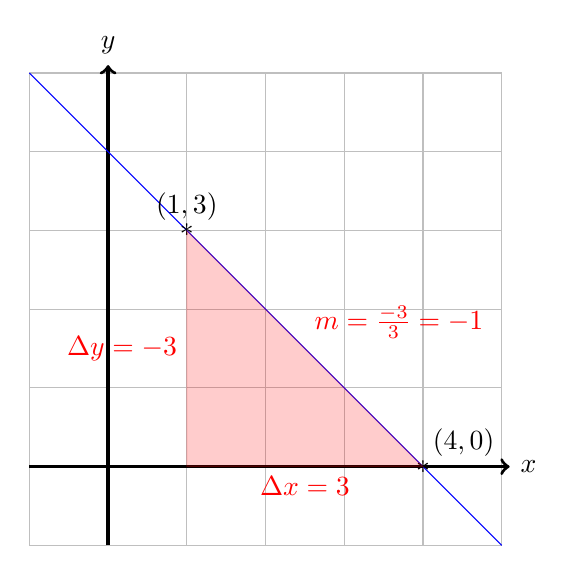
\begin{tikzpicture}[scale=1][domain=-1:5]
    \draw[gray!50, thin, step=1] (-1,-1) grid (5,5);
    \draw[very thick,->] (-1,0) -- (5.1,0) node[right] {$x$};
    \draw[very thick,->] (0,-1) -- (0,5.1) node[above] {$y$};

%    \foreach \x in {0,...,11} \draw (\x,0.05) -- (\x,-0.05) node[below] {\tiny\x};
%    \foreach \y in {0,...,28} \draw (-0.05,\y) -- (0.05,\y) node[right] {\tiny\y};


  \draw[scale=1,domain=-1:5,smooth,variable=\x,blue] plot ({\x},{-1*\x+4});

\node at (1,3){$*$};
\draw (1,3) --node[above]{$(1,3)$}(1,3);

\node at (4,0){$*$};
\draw (4,0) --node[above right]{$(4,0)$}(4,0);

\draw[red, fill, opacity=0.2] (1,3)--(4,0)--(1,0)--(1,3);

\draw[red] (1,1.5) --node[left]{$\Delta y =-3$}(1,1.5);

\draw[red] (2.5,0) --node[below]{$\Delta x =3$}(2.5,0);

\draw[red] (2.5,1.5) --node[above right]{$m=\frac{-3}{3}=-1$}(2.5,1.5);




\end{tikzpicture}%
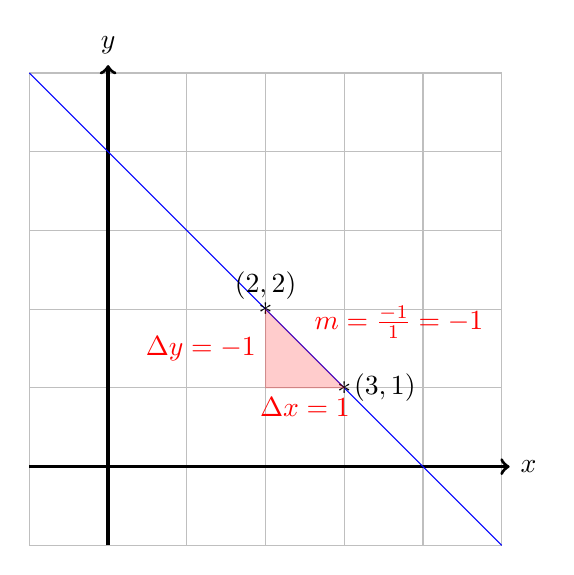
\begin{tikzpicture}[scale=1][domain=-1:5]
    \draw[gray!50, thin, step=1] (-1,-1) grid (5,5);
    \draw[very thick,->] (-1,0) -- (5.1,0) node[right] {$x$};
    \draw[very thick,->] (0,-1) -- (0,5.1) node[above] {$y$};

%    \foreach \x in {0,...,11} \draw (\x,0.05) -- (\x,-0.05) node[below] {\tiny\x};
%    \foreach \y in {0,...,28} \draw (-0.05,\y) -- (0.05,\y) node[right] {\tiny\y};


  \draw[scale=1,domain=-1:5,smooth,variable=\x,blue] plot ({\x},{-1*\x+4});

\node at (2,2){$*$};
\draw (2,2) --node[above]{$(2,2)$}(2,2);

\node at (3,1){$*$};
\draw (3,1) --node[right]{$(3,1)$}(3,1);

\draw[red, fill, opacity=0.2] (2,2)--(3,1)--(2,1)--(2,2);

\draw[red] (2,1.5) --node[left]{$\Delta y =-1$}(2,1.5);

\draw[red] (2.5,1) --node[below]{$\Delta x =1$}(2.5,1);

\draw[red] (2.5,1.5) --node[above right]{$m=\frac{-1}{1}=-1$}(2.5,1.5);




\end{tikzpicture}$$ % of mbox


An interactive version of this graph can be found here:  \url{https://www.desmos.com/calculator/9s3kfotxne}.



\end{example}

\begin{example}\label{Example:NullSlope}
Let $y=3$.  We can re-imagine this as $y=0x+3$, so this represents a linear function with $m=0$ and $b=3$.  Note that no matter what the $x$ values are, $y=3$.  So $\Delta y=0$, and $m=\frac{\Delta y}{\Delta x}=\frac{0}{\Delta x}=0$.  Intuitively, $y$ is always 3 and never changes, so the ``rate of change" is a constant nothing.  This gives us a horizontal line.

This can be represented visually:

$$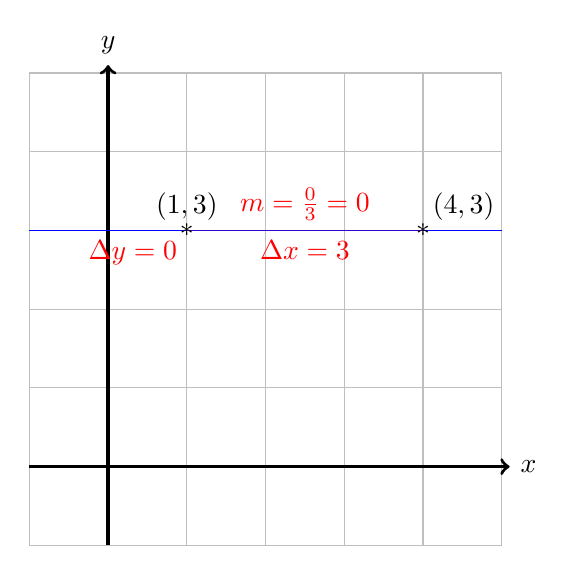
\begin{tikzpicture}[scale=1][domain=-1:5]
    \draw[gray!50, thin, step=1] (-1,-1) grid (5,5);
    \draw[very thick,->] (-1,0) -- (5.1,0) node[right] {$x$};
    \draw[very thick,->] (0,-1) -- (0,5.1) node[above] {$y$};


  \draw[scale=1,domain=-1:5,smooth,variable=\x,blue] plot ({\x},{3});

\node at (1,3){$*$};
\draw (1,3) --node[above]{$(1,3)$}(1,3);

\node at (4,3){$*$};
\draw (4,3) --node[above right]{$(4,3)$}(4,3);

\draw[red, opacity=0.2] (1,3)--(4,3);

\draw[red] (1,3) --node[below left]{$\Delta y =0$}(1,3);

\draw[red] (2.5,3) --node[below]{$\Delta x =3$}(2.5,3);

\draw[red] (2.5,3) --node[above]{$m=\frac{0}{3}=0$}(2.5,3);



\end{tikzpicture}%
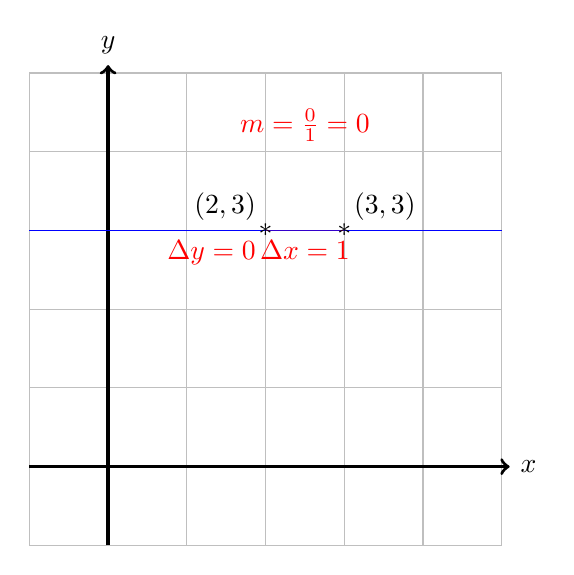
\begin{tikzpicture}[scale=1][domain=-1:5]
    \draw[gray!50, thin, step=1] (-1,-1) grid (5,5);
    \draw[very thick,->] (-1,0) -- (5.1,0) node[right] {$x$};
    \draw[very thick,->] (0,-1) -- (0,5.1) node[above] {$y$};


  \draw[scale=1,domain=-1:5,smooth,variable=\x,blue] plot ({\x},{3});

\node at (2,3){$*$};
\draw (2,3) --node[above left]{$(2,3)$}(2,3);

\node at (3,3){$*$};
\draw (3,3) --node[above right]{$(3,3)$}(3,3);

\draw[red, opacity=0.2] (2,3)--(3,3);

\draw[red] (2,3) --node[below left]{$\Delta y =0$}(2,3);

\draw[red] (2.5,3) --node[below]{$\Delta x =1$}(2.5,3);

\draw[red] (2.5,4) --node[above]{$m=\frac{0}{1}=0$}(2.5,4);




\end{tikzpicture}%
$$ % of mbox


An interactive version of this graph can be found here:  \url{https://www.desmos.com/calculator/pv7m6fbugb}.



\end{example}

\subsection{$\mathbf{y}$-intercept.}

The $\mathbf{y}$\textbf{-intercept} of a linear function $y=mx+b$ is the value $b$.  It is so named because it is the value of the linear function when it \textbf{intercepts} the $y$-axis.  The reason for this is that the $y$-axis is exactly the line $x=0$, and when $x=0$, $y=m(0)+b=b$.


\begin{example}\label{Example:Intercept}
Let us recall Example \ref{Example:Slope} and let $y=-x+4$.  Note that when $x=0, y=-(0)+4=4$.

This can be represented visually:

$$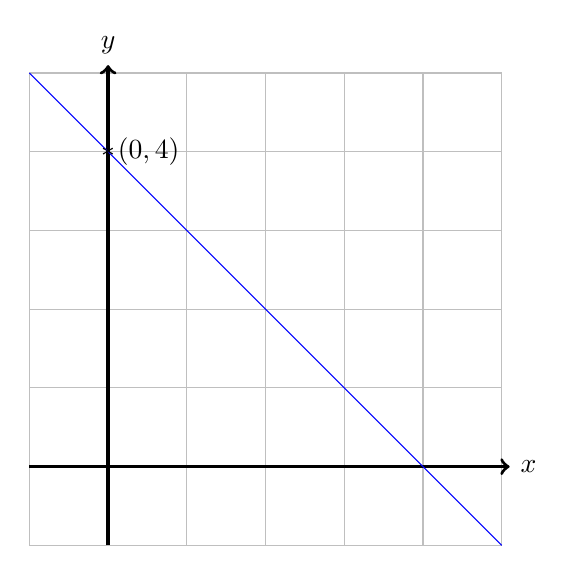
\begin{tikzpicture}[scale=1][domain=-1:5]
    \draw[gray!50, thin, step=1] (-1,-1) grid (5,5);
    \draw[very thick,->] (-1,0) -- (5.1,0) node[right] {$x$};
    \draw[very thick,->] (0,-1) -- (0,5.1) node[above] {$y$};

%    \foreach \x in {0,...,11} \draw (\x,0.05) -- (\x,-0.05) node[below] {\tiny\x};
%    \foreach \y in {0,...,28} \draw (-0.05,\y) -- (0.05,\y) node[right] {\tiny\y};


  \draw[scale=1,domain=-1:5,smooth,variable=\x,blue] plot ({\x},{-1*\x+4});

\node at (0,4){$*$};
\draw (0,4) --node[right]{$(0,4)$}(0,4);





\end{tikzpicture}$$ % of mbox


Note that $4$ is the height of the function when it intercepts the $y$-axis.


\end{example}

\begin{example}\label{Example:Intercept}
Let us recall Example \ref{Example:NullSlope} and let $y=3=0x+3$.  Note that when $x=0, y=3$.

This can be represented visually:

$$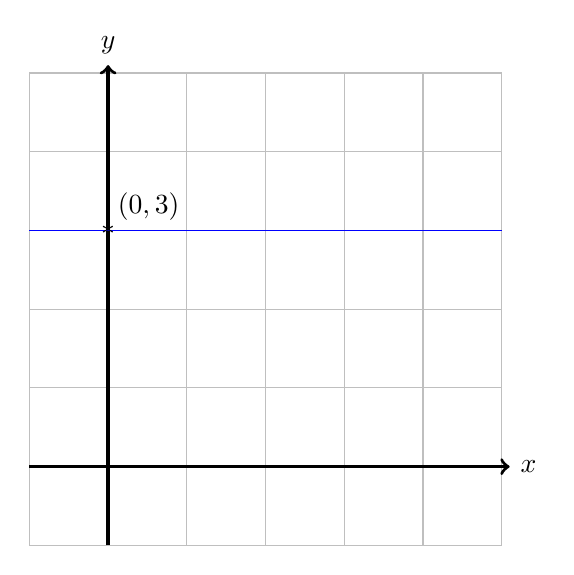
\begin{tikzpicture}[scale=1][domain=-1:5]
    \draw[gray!50, thin, step=1] (-1,-1) grid (5,5);
    \draw[very thick,->] (-1,0) -- (5.1,0) node[right] {$x$};
    \draw[very thick,->] (0,-1) -- (0,5.1) node[above] {$y$};

%    \foreach \x in {0,...,11} \draw (\x,0.05) -- (\x,-0.05) node[below] {\tiny\x};
%    \foreach \y in {0,...,28} \draw (-0.05,\y) -- (0.05,\y) node[right] {\tiny\y};


  \draw[scale=1,domain=-1:5,smooth,variable=\x,blue] plot ({\x},{3});

\node at (0,3){$*$};
\draw (0,3) --node[above right]{$(0,3)$}(0,3);





\end{tikzpicture}$$ % of mbox


Note that $3$ is the height of the function when it intercepts the $y$-axis.


\end{example}


\subsection{Translating from Algebra to Geometry}

We can see in our above examples that linear functions have both an algebraic form and a geometric interpretation.   Both are useful and in fact necessary to understand what's going on with a linear function.  So what we now want to ask ourselves is, given the algebraic expression for a line, how might we find it's geometric representation?\\


Intuitively, we know that if we had a sheet of paper and a ruler, if we drew 2 points on this paper, we could find the line between them.  So to find a geometric representation of a linear function, we should:

\begin{enumerate}
    \item Find a point that must be on thee line.
    \item Identify a second point on the line.
    \item Draw the line between them.
\end{enumerate}

\begin{example}\label{Example:DrawLine}
\textbf{Question:} Draw the line $y=f(x)$ where $f(x)=-\frac{2}{3}x+4$.

\begin{enumerate}
    \item We first identify a point on the line, the easiest to find is probably the $y$-intercept, note that when $x=0, f(x)=-\frac{2}{3}(0)+4=4$, thus $(0,4)$ is on $y=f(x)$.
    \item We have infinitely many choices for a second point, but to make the arithmetic easy, let's let $x=3$, then $f(x)=-\frac{2}{3}(3)+4=-2+4=2$, so $(3,2)$ is on the line.
    
    Note this gives us:
 $$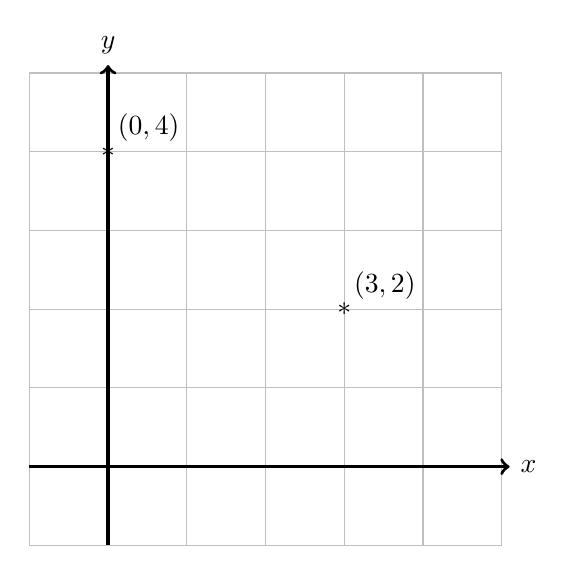
\begin{tikzpicture}[scale=1][domain=-1:5]
    \draw[gray!50, thin, step=1] (-1,-1) grid (5,5);
    \draw[very thick,->] (-1,0) -- (5.1,0) node[right] {$x$};
    \draw[very thick,->] (0,-1) -- (0,5.1) node[above] {$y$};

%    \foreach \x in {0,...,11} \draw (\x,0.05) -- (\x,-0.05) node[below] {\tiny\x};
%    \foreach \y in {0,...,28} \draw (-0.05,\y) -- (0.05,\y) node[right] {\tiny\y};


%  \draw[scale=1,domain=-1:5,smooth,variable=\x,blue] plot ({\x},{(-2/3)*\x+4});

\node at (0,4){$*$};
\draw (0,4) --node[above right]{$(0,4)$}(0,4);

\node at (3,2){$*$};
\draw (3,2) --node[above right]{$(3,2)$}(3,2);




\end{tikzpicture}$$    
    \item We then literally connect the dots:
$$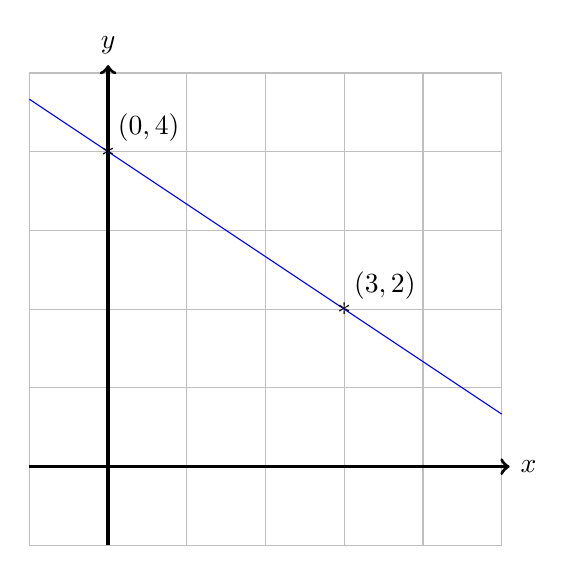
\begin{tikzpicture}[scale=1][domain=-1:5]
    \draw[gray!50, thin, step=1] (-1,-1) grid (5,5);
    \draw[very thick,->] (-1,0) -- (5.1,0) node[right] {$x$};
    \draw[very thick,->] (0,-1) -- (0,5.1) node[above] {$y$};

%    \foreach \x in {0,...,11} \draw (\x,0.05) -- (\x,-0.05) node[below] {\tiny\x};
%    \foreach \y in {0,...,28} \draw (-0.05,\y) -- (0.05,\y) node[right] {\tiny\y};


  \draw[scale=1,domain=-1:5,smooth,variable=\x,blue] plot ({\x},{(-2/3)*\x+4});

\node at (0,4){$*$};
\draw (0,4) --node[above right]{$(0,4)$}(0,4);

\node at (3,2){$*$};
\draw (3,2) --node[above right]{$(3,2)$}(3,2);




\end{tikzpicture}$$      
\end{enumerate}
Modern technology also let's us readily draw these functions: \url{https://www.desmos.com/calculator/gyvulordwz}.
\end{example}

\begin{example}\label{Example:DrawLineOtherForm}
\textbf{Question:} Draw the line $2x+4y=8$.

\begin{enumerate}
    \item We first identify a point on the line.  To make life easy note that when $x=0, 2(0)+4y=8$ and $y=2$, thus $(0,2)$ is on $2x+4y=8$.
    \item Similarly when $y=0, 2x+4(0)=8$ and $x=4$, thus $(4,0)$ is on $2x+4y=8$.
    
    Note this gives us:
 $$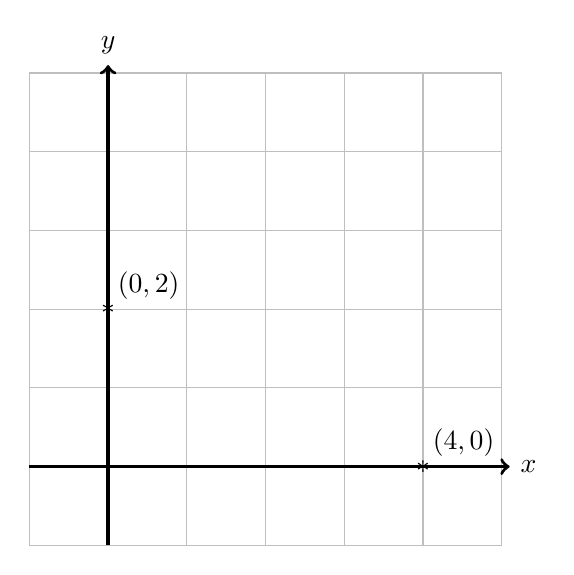
\begin{tikzpicture}[scale=1][domain=-1:5]
    \draw[gray!50, thin, step=1] (-1,-1) grid (5,5);
    \draw[very thick,->] (-1,0) -- (5.1,0) node[right] {$x$};
    \draw[very thick,->] (0,-1) -- (0,5.1) node[above] {$y$};

%    \foreach \x in {0,...,11} \draw (\x,0.05) -- (\x,-0.05) node[below] {\tiny\x};
%    \foreach \y in {0,...,28} \draw (-0.05,\y) -- (0.05,\y) node[right] {\tiny\y};


%  \draw[scale=1,domain=-1:5,smooth,variable=\x,blue] plot ({\x},{(-1/2)*\x+2});

\node at (0,2){$*$};
\draw (0,2) --node[above right]{$(0,2)$}(0,2);

\node at (4,0){$*$};
\draw (4,0) --node[above right]{$(4,0)$}(4,0);




\end{tikzpicture}$$    
    \item We then connect the dots:
$$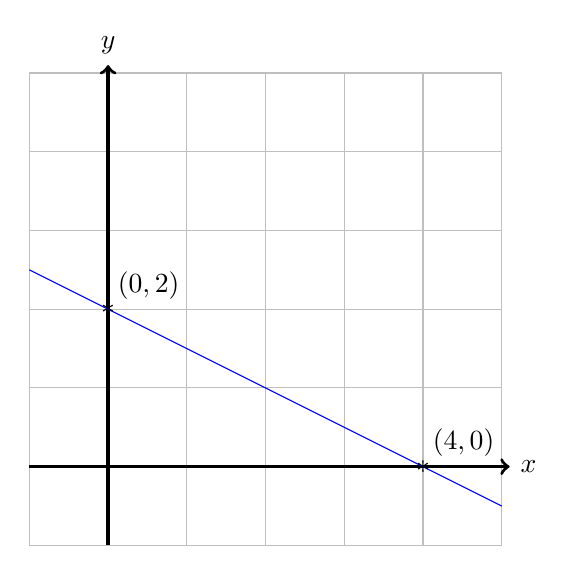
\begin{tikzpicture}[scale=1][domain=-1:5]
    \draw[gray!50, thin, step=1] (-1,-1) grid (5,5);
    \draw[very thick,->] (-1,0) -- (5.1,0) node[right] {$x$};
    \draw[very thick,->] (0,-1) -- (0,5.1) node[above] {$y$};

%    \foreach \x in {0,...,11} \draw (\x,0.05) -- (\x,-0.05) node[below] {\tiny\x};
%    \foreach \y in {0,...,28} \draw (-0.05,\y) -- (0.05,\y) node[right] {\tiny\y};


  \draw[scale=1,domain=-1:5,smooth,variable=\x,blue] plot ({\x},{(-1/2)*\x+2});

\node at (0,2){$*$};
\draw (0,2) --node[above right]{$(0,2)$}(0,2);

\node at (4,0){$*$};
\draw (4,0) --node[above right]{$(4,0)$}(4,0);




\end{tikzpicture}$$          
\end{enumerate}
Again, utilizing technology: \url{https://www.desmos.com/calculator/lprlevpf6q}.\\

Note that we could have taken $2x+4y=8$ and rewritten it:

\begin{eqnarray*}
2x+4y&=&8\\
4y&=&-2x+8\\
y&=&-\frac{1}{2}x+2,
\end{eqnarray*}

and from here, treated it the same way as in Example \ref{Example:DrawLine}.

\end{example}



\section{Identifying a Linear Function from information.}


It is often the case that when one works with a linear function, one will not be given the exact form for the function.  You may for example only know the rate of change, or the value of the function at a few points.  To be able to make the most of this situation, it would be good to be able to still identify the linear function in question, when possible.\\

\textbf{Question:}  What is the minimal amount of information necessary to identify a linear function?\\

Here is where our geometric interpretation of these functions is helpful.  If someone handed you a sheet of paper and asked you to draw a line, how much information would they have to give you so there could be only one like you'd be able to draw?\\

\textbf{Question:}  Is a point enough?\\

If someone drew a dot on a piece of paper, there is certainly a line you could draw through it, but it definitely does seem like there's infinitely many lines you could draw as well.  Take $(2,3)$:

$$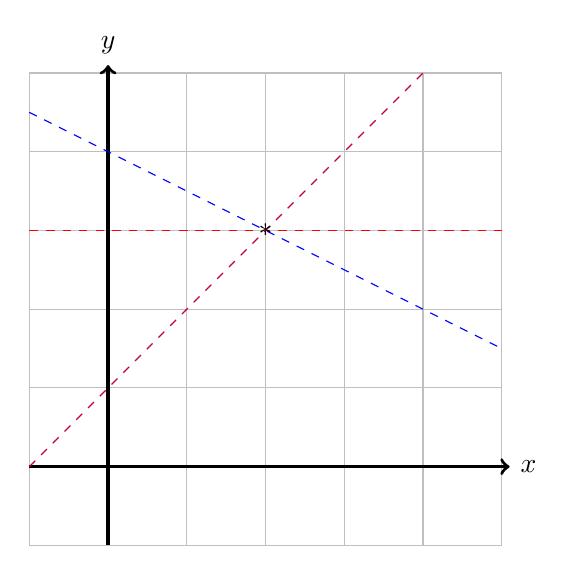
\begin{tikzpicture}[scale=1][domain=-1:5]
    \draw[gray!50, thin, step=1] (-1,-1) grid (5,5);
    \draw[very thick,->] (-1,0) -- (5.1,0) node[right] {$x$};
    \draw[very thick,->] (0,-1) -- (0,5.1) node[above] {$y$};

%    \foreach \x in {0,...,11} \draw (\x,0.05) -- (\x,-0.05) node[below] {\tiny\x};
%    \foreach \y in {0,...,28} \draw (-0.05,\y) -- (0.05,\y) node[right] {\tiny\y};


    \draw[scale=1,domain=-1:5,smooth,variable=\x,blue, dashed] plot ({\x},{(-1/2)*\x+4});
  
    \draw[scale=1,domain=-1:5,smooth,variable=\x,red, dashed] plot ({\x},{3});
    
    \draw[scale=1,domain=-1:4,smooth,variable=\x,purple, dashed] plot ({\x},{\x+1});

\node at (2,3){$*$};

\end{tikzpicture}$$   

Of course there are many more, here's a visualization: \url{https://www.desmos.com/calculator/c3gronrfd3}.



\textbf{Question:}  Is a slope/direction enough?\\

If someone gave you a piece of paper and told you would direction the line should take, there is definitely a line you could draw with that direction, but depending where you start, there's infinitely many lines you could draw as well.  Take $m=\frac{3}{2}$:

$$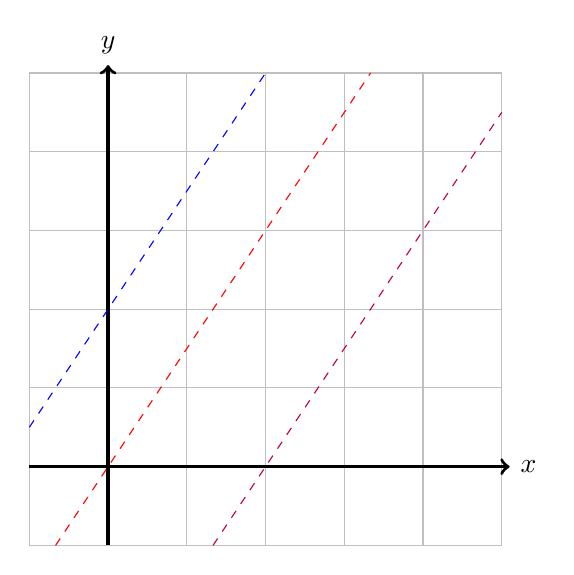
\begin{tikzpicture}[scale=1][domain=-1:5]
    \draw[gray!50, thin, step=1] (-1,-1) grid (5,5);
    \draw[very thick,->] (-1,0) -- (5.1,0) node[right] {$x$};
    \draw[very thick,->] (0,-1) -- (0,5.1) node[above] {$y$};

%    \foreach \x in {0,...,11} \draw (\x,0.05) -- (\x,-0.05) node[below] {\tiny\x};
%    \foreach \y in {0,...,28} \draw (-0.05,\y) -- (0.05,\y) node[right] {\tiny\y};


    \draw[scale=1,domain=-1:2,smooth,variable=\x,blue, dashed] plot ({\x},{(3/2)*\x+2});
  
    \draw[scale=1,domain=-2/3:10/3,smooth,variable=\x,red, dashed] plot ({\x},{(3/2)*\x});
    
    \draw[scale=1,domain=4/3:5,smooth,variable=\x,purple, dashed] plot ({\x},{(3/2)*\x-3});


\end{tikzpicture}$$   

Of course there are many more, here's a visualization: \url{https://www.desmos.com/calculator/iwcjwhen1b}.


So this begs the question, what \textbf{IS} the mininum amount of information that you'd need to uniquely identify a line?

\subsection{Point \& Slope}

If we combined the two pieces of information from the start of the section, would we obtain a unique line?  Intuitively this should make sense, there are infinitely many lines which go through a point, but only one with slope $m=\frac{3}{2}$, similarly, there are infinitely many lines with slope $\frac{3}{2}$, but they all pass through different points, only one of them passes through $(2,3)$.  Again to refer to our geometric ideas, if someone drew a point on a paper, and told you which direction you had to go from there, there's really only one line you could draw.\\

Here are some visualizations:  

$$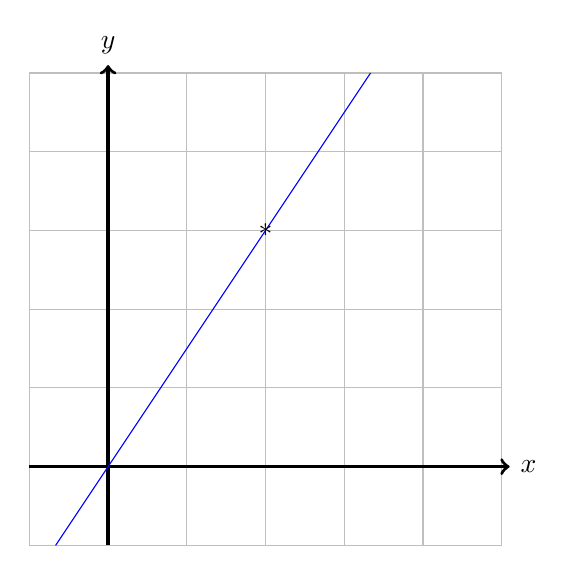
\begin{tikzpicture}[scale=1][domain=-1:5]
    \draw[gray!50, thin, step=1] (-1,-1) grid (5,5);
    \draw[very thick,->] (-1,0) -- (5.1,0) node[right] {$x$};
    \draw[very thick,->] (0,-1) -- (0,5.1) node[above] {$y$};



%    \foreach \x in {0,...,11} \draw (\x,0.05) -- (\x,-0.05) node[below] {\tiny\x};
%    \foreach \y in {0,...,28} \draw (-0.05,\y) -- (0.05,\y) node[right] {\tiny\y};


    \draw[scale=1,domain=-2/3:10/3,smooth,variable=\x,blue] plot ({\x},{(3/2)*\x});
  

\node at (2,3){$*$};

\end{tikzpicture}$$   



\url{https://www.desmos.com/calculator/5ikul0ktn5}, \url{https://www.desmos.com/calculator/hcl8ynd0yp}.

\textbf{Question:} How does this translate Algebraically?

So given a linear function is defined by the slope $m$ and intercept $b$.  By the discussion above, if we are given a slope $\textcolor{red}{m}$ and a pair of points $\textcolor{blue}{(x_0,y_0)}$, we should be able to uniquely identify $b$.

\begin{example}\label{Example:PandS}
\textbf{Question:}  Find the linear function with slope 3 passing through $(2,5)$.\\

Note that we are given $\textcolor{red}{m=3}$ and $\textcolor{blue}{(x_0,y_0)=(2,5)}$.  The general form for a line is $y=mx+b$, thus:

\begin{eqnarray*}
y&=&mx+b\\
\textcolor{blue}{5}&=&\textcolor{red}{3}\cdot\textcolor{blue}{2}+b\\
5&=&6+b\\
b&=&5-6=-1.\\
\end{eqnarray*}

Thus $y=3x-1$ is the linear equation in question, $m=3, b=-1$.

$$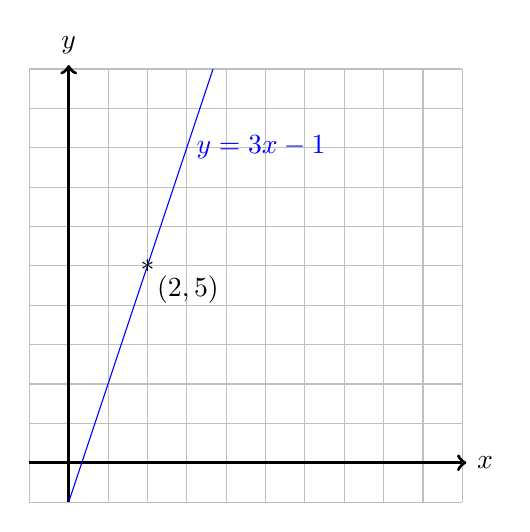
\begin{tikzpicture}[scale=0.5][domain=-1:10]
    \draw[gray!50, thin, step=1] (-1,-1) grid (10,10);
    \draw[very thick,->] (-1,0) -- (10.1,0) node[right] {$x$};
    \draw[very thick,->] (0,-1) -- (0,10.1) node[above] {$y$};

%    \foreach \x in {0,...,11} \draw (\x,0.05) -- (\x,-0.05) node[below] {\tiny\x};
%    \foreach \y in {0,...,28} \draw (-0.05,\y) -- (0.05,\y) node[right] {\tiny\y};


    \draw[scale=1,domain=0:3.666,smooth,variable=\x,blue] plot ({\x},{(3)*\x-1});
  

\node at (2,5){$*$};
\draw (2,5) --node[below right]{$(2,5)$}(2,5);
\draw[blue] (3,8) --node[right]{$y=3x-1$}(3,8);



\end{tikzpicture}$$   
\url{https://www.desmos.com/calculator/w3nixbtfrs}.

We can verify that this line has slope $m=3$ and when $x=2, y=3\cdot 2-1=6-1=5$.

\end{example}


\subsection{Point-Slope form.}

So, typically lines are defined in the form $y=mx+b$, where $m$ is the slope and $b$ is the $y$-intercept.  It can be convenient to also define a line in the form $$y-y_0=m(x-x_0),$$ where $(x_0, y_0)$ is a point that falls on your line.\\

Why would we care about a second formulation, and how do we know it's even a line?  To answer the first question, we recall that ANY geometric object defined by an equation is the set of points that make the equation true.  So given the equation $y-y_0=m(x-x_0)$, if we plug in $(x_0, y_0)$, we would get $y_0-y_0=m(x_0-x_0)$ or $0=0$ which is definitely a true statement.  So whatever shape we get from $y-y_0=m(x-x_0)$, it contains $(x_0, y_0)$.\\

We know it's a line because:

\begin{eqnarray*}
y-y_0&=&m(x-x_0)\\
y&=&mx-mx_0+y_0\\
y&=&mx+(y_0-mx_0)
\end{eqnarray*}

so if we let $b=y_0-mx_0$, we get the standard form for a line.


\begin{example}\label{Example:PandSagain}
\textbf{Question:} Find the line with slope 3 passing through $(2,5)$, again.\\

Using the point-slope form, knowing that $\textcolor{blue}{(2,5)}$ lies on the line, and that $\textcolor{red}{m}$:

\begin{eqnarray*}
y-y_0&=&m(x-x_0)\\
y-\textcolor{blue}{5}&=&\textcolor{red}{3}(x-\textcolor{blue}{2})\\
y&=&3x-6+5\\
y&=&3x-1.
\end{eqnarray*}

Either way, you obtain the same line, with slope 3, passing through (2,5).

\end{example}

\subsection{Two Points}

On the other hand, instead of giving you a point and a direction, one could be given two points to traverse through.  If you imagine any two dots on a piece of paper, one can imagine that you may draw a line between them.  The exact way we do this also follows intuitively.  If you were at home, and you had to go to the store, the natural steps you would take to do so are:

\begin{enumerate}
\item Figure out which way to the store.
\item Go there.
\end{enumerate}

So we have to figure out the direction between these points, which in our analogy means the slope between the points.  Remember the slope measures how much $y$ changes per change in $x$, or $m=\frac{\Delta y}{\Delta x}$.  So, the measurement of slope follows from the change in $y$ over the change in $x$.  So to measure this, if we have points $(x_0, y_0), (x_1, y_1)$, we want to see how much $y$ changes over how much $x$ changes, or:

$$m=\frac{\Delta y}{\Delta x}=\frac{y_1-y_0}{x_1-x_0}$$
or equivalently $m=\frac{y_0-y_1}{x_0-x_1}$.


\begin{example}\label{Example:PandP}
What line passes between $(2,3)$ and $(4,1)$?\\

So we note then that $\textcolor{red}{m=\frac{1-3}{4-2}=-1}$ (also $\textcolor{red}{m=\frac{3-1}{2-4}=-1}$).  Once the slope is identified, we can use any point, and any method to find the line.  Once we pick a point, We have a problem that follows the form of Examples \ref{Example:PandS}, \ref{Example:PandSagain}.

We won't go through all the possibilities but if we considered the point $\textcolor{blue}{(2,3)}$:

\begin{eqnarray*}
y&=&mx+b\\
\textcolor{blue}{3}&=&\textcolor{red}{-1}\cdot \textcolor{blue}{2}+b\\
b&=&3+2=5\\
y&=&-x+5.
\end{eqnarray*}

Or if we picked $\textcolor{blue}{(1,4)}$:

\begin{eqnarray*}
y-y_0&=&m(x-x_0)\\
y-\textcolor{blue}{1}&=&\textcolor{red}{-1}\cdot(x-\textcolor{blue}{4})\\
y&=&-x+4+1\\
y&=&-x+5.
\end{eqnarray*}

Either way, we identify the same line:

$$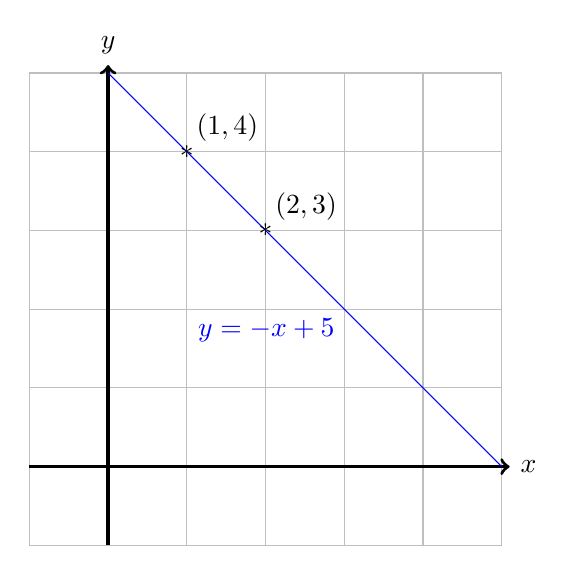
\begin{tikzpicture}[scale=1][domain=-1:5]
    \draw[gray!50, thin, step=1] (-1,-1) grid (5,5);
    \draw[very thick,->] (-1,0) -- (5.1,0) node[right] {$x$};
    \draw[very thick,->] (0,-1) -- (0,5.1) node[above] {$y$};

%    \foreach \x in {0,...,11} \draw (\x,0.05) -- (\x,-0.05) node[below] {\tiny\x};
%    \foreach \y in {0,...,28} \draw (-0.05,\y) -- (0.05,\y) node[right] {\tiny\y};


    \draw[scale=1,domain=0:5,smooth,variable=\x,blue] plot ({\x},{(-1)*\x+5});
  

\node at (2,3){$*$};
\draw (2,3) --node[above right]{$(2,3)$}(2,3);

\node at (1,4){$*$};
\draw (1,4) --node[above right]{$(1,4)$}(1,4);

\draw[blue] (3,2) --node[below left]{$y=-x+5$}(3,2);


\end{tikzpicture}$$  

\url{https://www.desmos.com/calculator/yohrdbuwuc}

\end{example}

\section{Utilizing the Linear Function}

Once you obtain a linear function, this gives you a relationship between the $x$ and $y$ variables.  It allows you to identify, given an $x$ or $y$ value, the other value:

\begin{example}\label{Example:LinearFindValue}
Consider the linear function $y=2x-3$.
\begin{enumerate}
\item When $y=0$, what is $x$?
\item When $x=3$ what is $y$?
\end{enumerate}

These can be identified algebraically:
\begin{enumerate}
\item When $\textcolor{ForestGreen}{y=0}$, we have:
\begin{eqnarray*}
y&=&2x-3\\
\textcolor{ForestGreen}{0}&=&2x-3\\
3&=&2x\\
x&=&1.5.
\end{eqnarray*}
\item If $\textcolor{orange}{x=3}$:
\begin{eqnarray*}
y&=&2x-3\\
y&=&2(\textcolor{orange}{3})-3\\
y&=&6-3=3.
\end{eqnarray*}
We can identify both points graphically as well:



\url{https://www.desmos.com/calculator/gukgr4sjfm}.
\end{enumerate}

$$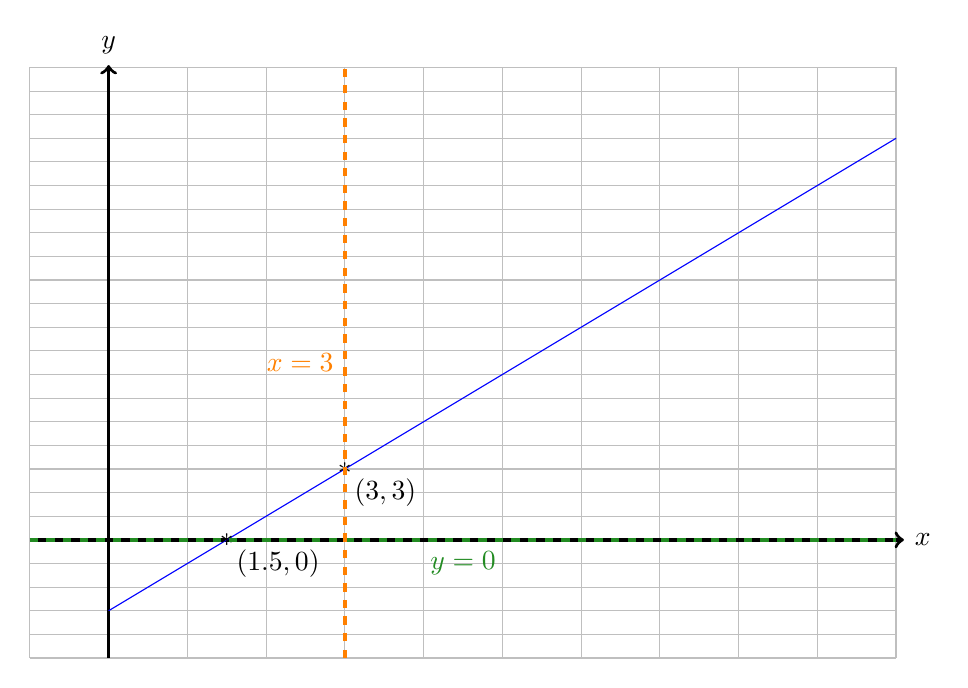
\begin{tikzpicture}[yscale=0.3][domain=-1:10]
    \draw[gray!50, thin, step=1] (-1,-5) grid (10,20);
    \draw[very thick,->] (-1,0) -- (10.1,0) node[right] {$x$};
    \draw[very thick,->] (0,-5) -- (0,20.1) node[above] {$y$};

%    \foreach \x in {0,...,11} \draw (\x,0.05) -- (\x,-0.05) node[below] {\tiny\x};
%    \foreach \y in {0,...,28} \draw (-0.05,\y) -- (0.05,\y) node[right] {\tiny\y};


    \draw[scale=1,domain=0:10,smooth,variable=\x,blue] plot ({\x},{(2)*\x-3});
  

\node at (1.5,0){$*$};
\draw (1.5,0) --node[below right]{$(1.5,0)$}(1.5,0);

\node at (3,3){$*$};
\draw (3,3) --node[below right]{$(3,3)$}(3,3);

\draw[ForestGreen, dashed, ultra thick] (-1,0) --node[below]{$y=0$}(10,0);

\draw[orange, dashed, ultra thick] (3,-5) --node[left]{$x=3$}(3,20);


\end{tikzpicture}$$  

\end{example}


\section{Applications of Linear Functions}

Up until this point, we've been treating linear functions as somewhat disembodied Mathematical entities.  In this section, we'll give a few examples to show how they appear and are applied in practice.


\begin{example}\label{Example:LinearTemp}

\Q The freezing point of water is $0^\circ$ Celsius and $32^\circ$ Fahrenheit.  The boiling point of water is $100^\circ$ Celsius and $212^\circ$ Fahrenheit.

\begin{enumerate}
    \item Find a linear function $T(F)=C$ that converts Fahrenheit into Celsius.
    \item When it's 10 degrees Fahrenheit, what is the temperature in Celsius?
    \item When it's 30 degrees Celsius, what is the temperature in Fahrenheit?
\end{enumerate}

\Sol We are given that $T(32)=0$ and $T(212)=100$.  This gives us points $(32,0)$ and $(212,100)$, so this bears some similarity to Example \ref{Example:PandP}.

\begin{enumerate}
    \item We first identify the slope of the function: $$m=\frac{\Delta C}{\Delta F}=\frac{100-0}{212-32}=\frac{100}{180}=\TCR{\frac{5}{9}}.$$
Then choosing either point, say $\TCB{(32,0)}$, and point slope form, we have:
\begin{eqnarray*}
C-C_0&=&m(F-F_0)\\
C-\TCB{0}&=&\TCR{\frac{5}{9}}(F-\TCB{32})\\
C&=&\frac{5}{9}F-\frac{160}{9}.
\end{eqnarray*}

Thus $T(F)=\frac{5}{9}F-\frac{160}{9}$

$$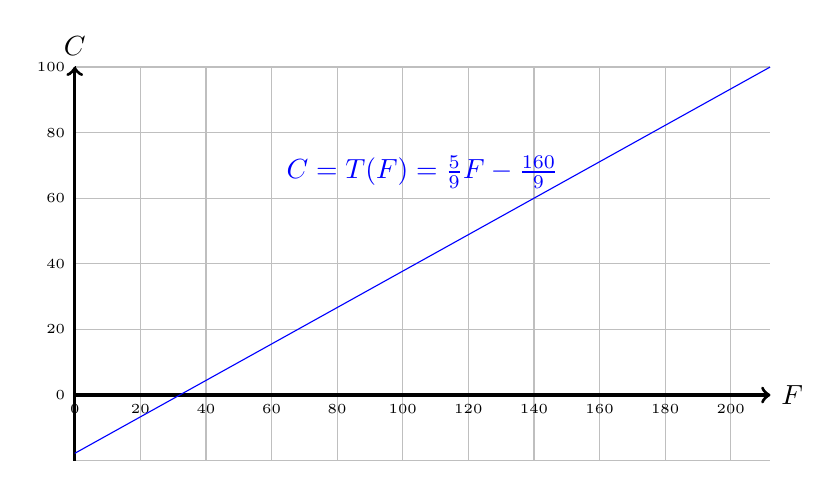
\begin{tikzpicture}[yscale=1/24, xscale=1/24][domain=-1:10]
    \draw[gray!50, thin, step=20] (0,-20) grid (212,100);
    \draw[very thick,->] (0,0) -- (212.1,0) node[right] {$F$};
    \draw[very thick,->] (0,-20) -- (0,100.1) node[above] {$C$};

    \foreach \x in {0,20,...,200} \draw (\x,0.05) -- (\x,-0.05) node[below] {\tiny\x};
    \foreach \y in {0,20,...,100} \draw (-0.05,\y) -- (0.05,\y) node[left] {\tiny\y};


    \draw[scale=1,domain=0:212,smooth,variable=\x,blue] plot ({\x},{(5/9)*\x-160/9});
  

\draw[blue] (106,60) --node[above]{$C=T(F)=\frac{5}{9}F-\frac{160}{9}$}(106,60);


\end{tikzpicture}$$ 

\item When it's 10 degrees, we have that $\TCG{F=10}$ and so:

\begin{eqnarray*}
C&=&\frac{5}{9}F-\frac{160}{9}\\
C&=&\frac{5}{9}\cdot\TCG{10}-\frac{160}{9}\\
C&=&\frac{50}{9}-\frac{160}{9}\\
C&=&-\frac{110}{9}\approx-12.2222.
\end{eqnarray*}
So 10 degrees Fahrenheit is $-\frac{110}{9}\approx-12.2222$ degrees Celsius.

$$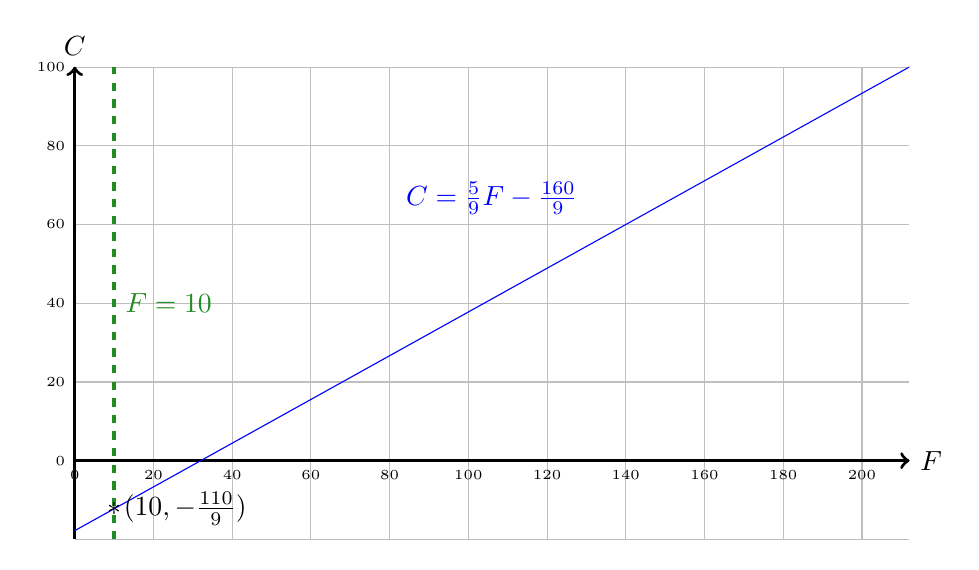
\begin{tikzpicture}[yscale=1/20, xscale=1/20][domain=-1:10]
    \draw[gray!50, thin, step=20] (0,-20) grid (212,100);
    \draw[very thick,->] (0,0) -- (212.1,0) node[right] {$F$};
    \draw[very thick,->] (0,-20) -- (0,100.1) node[above] {$C$};

    \foreach \x in {0,20,...,200} \draw (\x,0.05) -- (\x,-0.05) node[below] {\tiny\x};
    \foreach \y in {0,20,...,100} \draw (-0.05,\y) -- (0.05,\y) node[left] {\tiny\y};


    \draw[scale=1,domain=0:212,smooth,variable=\x,blue] plot ({\x},{(5/9)*\x-160/9});
  

\draw[blue] (106,60) --node[above]{$C=\frac{5}{9}F-\frac{160}{9}$}(106,60);
\draw[ultra thick, dashed, ForestGreen] (10,-20) --node[right]{$F=10$} (10,100);

\node at (10,-12.22222){$*$};
\draw (10,-12.22222) --node[right]{$(10,-\frac{110}{9})$}(10,-12.22222);



\end{tikzpicture}$$ 

\item When it's 30 degrees Celsius i.e.\ $\TCO{C=30}$ we have:

\begin{eqnarray*}
C&=&\frac{5}{9}F-\frac{160}{9}\\
\TCO{30}&=&\frac{5}{9}F-\frac{160}{9}\\
30+\frac{160}{9}&=&\frac{5}{9}F\\
\frac{430}{9}&=&\frac{5}{9}F\\
F&=&\frac{430}{5}=86.
\end{eqnarray*}

So when it's 30 degrees Celsius, it is 86 degrees Fahrenheit.

$$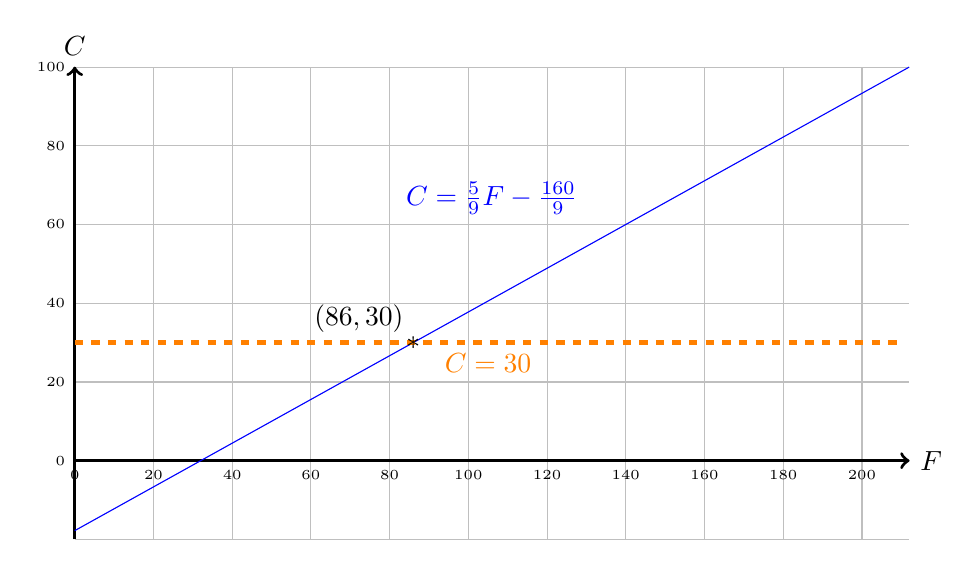
\begin{tikzpicture}[yscale=1/20, xscale=1/20][domain=-1:10]
    \draw[gray!50, thin, step=20] (0,-20) grid (212,100);
    \draw[very thick,->] (0,0) -- (212.1,0) node[right] {$F$};
    \draw[very thick,->] (0,-20) -- (0,100.1) node[above] {$C$};

    \foreach \x in {0,20,...,200} \draw (\x,0.05) -- (\x,-0.05) node[below] {\tiny\x};
    \foreach \y in {0,20,...,100} \draw (-0.05,\y) -- (0.05,\y) node[left] {\tiny\y};


    \draw[scale=1,domain=0:212,smooth,variable=\x,blue] plot ({\x},{(5/9)*\x-160/9});
  

\draw[blue] (106,60) --node[above]{$C=\frac{5}{9}F-\frac{160}{9}$}(106,60);
\draw[ultra thick, dashed, orange] (0,30) --node[below]{$C=30$} (210,30);

\node at (86,30){$*$};
\draw (86,30) --node[above left]{$(86,30)$}(86,30);



\end{tikzpicture}$$ 


\end{enumerate}

Desmos representation here: \url{https://www.desmos.com/calculator/tyoznzrk53}.


\end{example}

\begin{example}\label{Example:Proft}
\Q Suppose you were selling widgets for \$5 a unit, they have a marginal cost of \$3 per unit, and a fixed cost of production of \$20.

\begin{enumerate}
    \item Find the Cost, Revenue and Profit functions of producing $x$ widgets ($C(x), R(x), P(x)$) in dollars.
    \item For each widget sold, how much does your profit increase?
    \item  What is the cost of producing 30 widgets?
    \item What is the break even point?  (Zero profit).
\end{enumerate}

\Sol

\begin{enumerate}
    \item We break these down one at a time.
    \begin{enumerate}
        \item The marginal cost or cost per widget is \$3, and the cost for producing no widgets is the fixed cost of \$20.  Thus $C(x)=3x+20$.
        \item You get \$5 per widget sold, and clearly do not get any money for selling nothing, so $R(x)=5x+0=5x$.
        \item Profit is Revenue (money generated) minus Costs (money spent).  Thus $P(x)=R(x)-C(x)=5x-(3x+20)=2x-20$.
    \end{enumerate}
    $$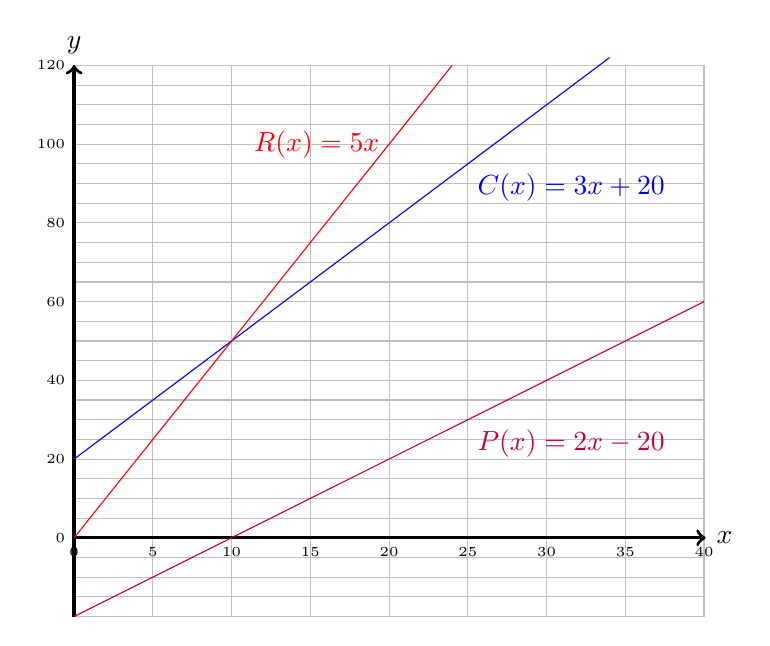
\begin{tikzpicture}[yscale=1/20, xscale=1/5]
    \draw[gray!50, thin, step=5] (0,-20) grid (40,120);
    \draw[very thick,->] (0,0) -- (40.1,0) node[right] {$x$};
    \draw[very thick,->] (0,-20) -- (0,120.1) node[above] {$y$};

    \foreach \x in {0,5,...,40} \draw (\x,0.05) -- (\x,-0.05) node[below] {\tiny\x};
    \foreach \y in {0,20,...,120} \draw (-0.05,\y) -- (0.05,\y) node[left] {\tiny\y};


    \draw[scale=1,domain=0:34,smooth,variable=\x,blue] plot ({\x},{3*\x+20});
  
    \draw[scale=1,domain=0:24,smooth,variable=\x,red] plot ({\x},{5*\x});

    \draw[scale=1,domain=0:40,smooth,variable=\x,purple] plot ({\x},{2*\x-20});

\draw[blue] (25,95) --node[below right]{$C(x)=3x+20$}(25,95);
\draw[red] (20,100) --node[left]{$R(x)=5x$}(20,100);
\draw[purple] (25,30) --node[below right]{$P(x)=2x-20$}(25,30);



\end{tikzpicture}$$ 

\url{https://www.desmos.com/calculator/d6l9b3kqho}

\item Since $P(x)=2x-20$, the change per unit of $x$ or profit per widget is the slope, or \$2/widget.

\item When you produce $\TCG{x=30}$ widgets, the cost will be:

\begin{eqnarray*}
C(x)&=&3x+20\\
C(x)&=&3\cdot\TCG{30}+20\\
C(x)&=&90+20\\
C(x)&=&110.\\
\end{eqnarray*}
The cost of producing 30 widgets is \$110.

 $$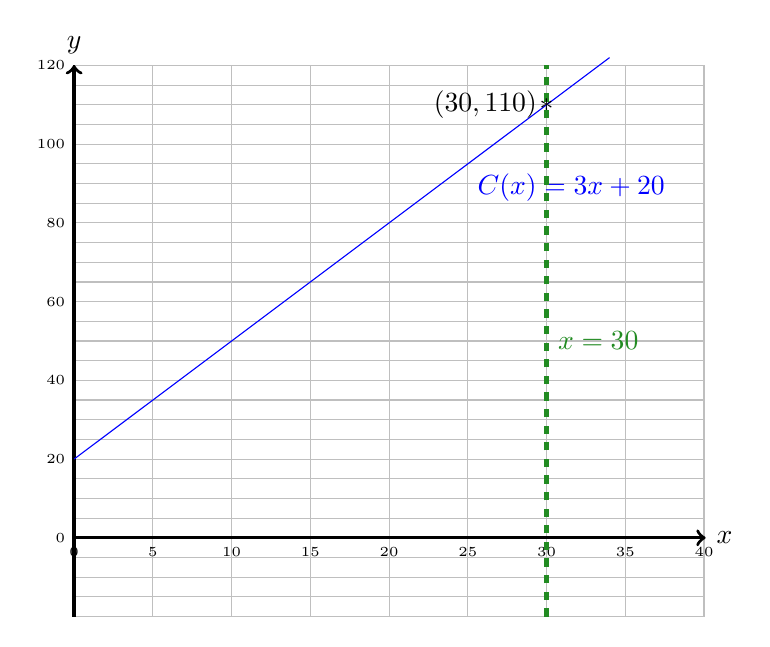
\begin{tikzpicture}[yscale=1/20, xscale=1/5]
    \draw[gray!50, thin, step=5] (0,-20) grid (40,120);
    \draw[very thick,->] (0,0) -- (40.1,0) node[right] {$x$};
    \draw[very thick,->] (0,-20) -- (0,120.1) node[above] {$y$};

    \foreach \x in {0,5,...,40} \draw (\x,0.05) -- (\x,-0.05) node[below] {\tiny\x};
    \foreach \y in {0,20,...,120} \draw (-0.05,\y) -- (0.05,\y) node[left] {\tiny\y};


    \draw[scale=1,domain=0:34,smooth,variable=\x,blue] plot ({\x},{3*\x+20});
  
%    \draw[scale=1,domain=0:24,smooth,variable=\x,red] plot ({\x},{5*\x});

%    \draw[scale=1,domain=0:40,smooth,variable=\x,purple] plot ({\x},{2*\x-20});

\draw[blue] (25,95) --node[below right]{$C(x)=3x+20$}(25,95);
%\draw[red] (20,100) --node[left]{$R(x)=5x$}(20,100);
%\draw[purple] (25,30) --node[below right]{$P(x)=2x-20$}(25,30);

\draw[ultra thick, dashed, ForestGreen] (30,-20) --node[right]{$x=30$} (30,120);

\node at (30,110){$*$};
\draw (30,110) --node[left]{$(30,110)$}(30,110);


\end{tikzpicture}$$ 
\url{https://www.desmos.com/calculator/cmoor2agyv}

\item The break even occurs when the profit is zero, $\TCO{P(x)=0}$.

\begin{eqnarray*}
P(x)&=&2x-20\\
\TCO{0}&=&2x-20\\
2x&=&20\\
x&=&10.
\end{eqnarray*}
The break even point occurs when $x=10$ widgets are sold.

 $$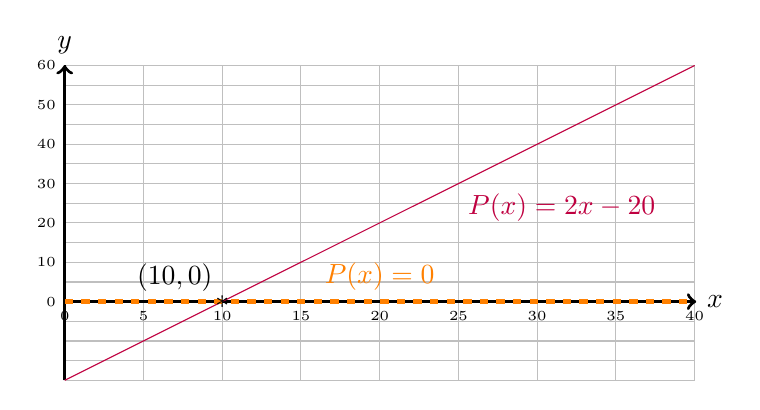
\begin{tikzpicture}[yscale=1/20, xscale=1/5]
    \draw[gray!50, thin, step=5] (0,-20) grid (40,60);
    \draw[very thick,->] (0,0) -- (40.1,0) node[right] {$x$};
    \draw[very thick,->] (0,-20) -- (0,60.1) node[above] {$y$};

    \foreach \x in {0,5,...,40} \draw (\x,0.05) -- (\x,-0.05) node[below] {\tiny\x};
    \foreach \y in {0,10,...,60} \draw (-0.05,\y) -- (0.05,\y) node[left] {\tiny\y};


%    \draw[scale=1,domain=0:34,smooth,variable=\x,blue] plot ({\x},{3*\x+20});
  
%    \draw[scale=1,domain=0:24,smooth,variable=\x,red] plot ({\x},{5*\x});

    \draw[scale=1,domain=0:40,smooth,variable=\x,purple] plot ({\x},{2*\x-20});

%\draw[blue] (25,95) --node[below right]{$C(x)=3x+20$}(25,95);
%\draw[red] (20,100) --node[left]{$R(x)=5x$}(20,100);
\draw[purple] (25,30) --node[below right]{$P(x)=2x-20$}(25,30);

\draw[ultra thick, dashed, orange] (0,0) --node[above]{$P(x)=0$} (40,0);

\node at (10,0){$*$};
\draw (10,0) --node[above left]{$(10,0)$}(10,0);


\end{tikzpicture}$$ 
\url{https://www.desmos.com/calculator/bdtdeqzqqa}

\end{enumerate}



\end{example}



\begin{example}
\Q Dr.\ Johnson is traveling to visit her mother for a holiday.  She drives at a constant speed of 75 mph.  After 3 hours, she passes a landmark that she knows is 200 miles from her mom's house.
\begin{enumerate}
    \item Find a function $D(t)$ that gives Dr.\ Johnson's distance to her mother house, in miles, after $t$ hours.
    \item How far away was she when she started driving?
    \item How many hours did it take from start to finish to complete this drive?
\end{enumerate}

\Sol 
\begin{enumerate}
    \item Since she is driving towards her mom's house, the distance from her to the house decreases at a rate of 75 miles per hour.  Thus $\TCR{m=-75}$.  At $t=3$ hours, her distance was 200 miles away.  Thus $\TCB{(3,200)}$ falls on the line representing this function.  Recall the techniques from Examples \ref{Example:PandS}, \ref{Example:PandSagain}.
     \begin{eqnarray*}
    D(t)&=&-75t+b\\
    \TCB{200}&=&\TCR{-75}\cdot\TCB{3}+b\\
    200&=&-225+b\\
    b&=&200+225=425.
    \end{eqnarray*}
    Thus $D(t)=-75t+425$.   
 $$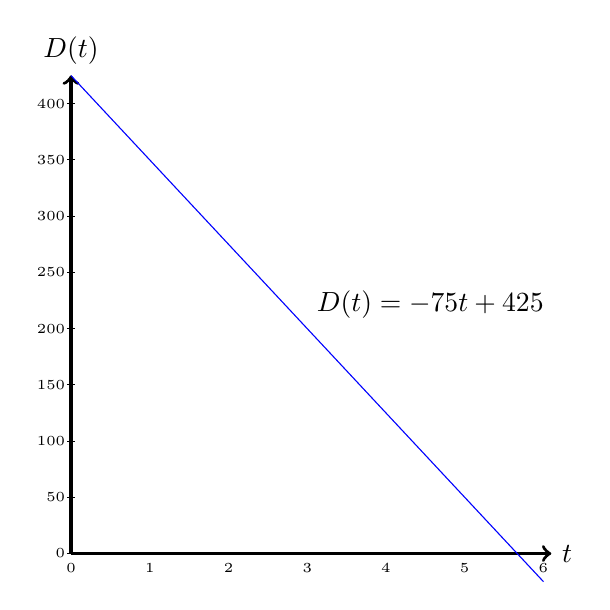
\begin{tikzpicture}[yscale=1/70]
    %\draw[gray!50, thin, step=5] (0,-20) grid (40,60);
    \draw[very thick,->] (0,0) -- (6.1,0) node[right] {$t$};
    \draw[very thick,->] (0,0) -- (0,425.1) node[above] {$D(t)$};

    \foreach \x in {0,1,...,6} \draw (\x,0.05) -- (\x,-0.05) node[below] {\tiny\x};
    \foreach \y in {0,50,...,425} \draw (-0.05,\y) -- (0.05,\y) node[left] {\tiny\y};



    \draw[scale=1,domain=0:6,smooth,variable=\x,blue] plot ({\x},{-75*\x+425});

\draw (3,200) --node[above right]{$D(t)=-75t+425$}(3,200);


%\node at (10,0){$*$};
%\draw (10,0) --node[above left]{$(10,0)$}(10,0);


\end{tikzpicture}$$ 
\url{https://www.desmos.com/calculator/uoul2cdsjs}
    \item At the start of the journey, $\TCG{t=0}$, and so she was $D(\TCG{0})=-75\cdot\TCG{0}+425=425$ miles from her mother's house.
\url{https://www.desmos.com/calculator/xuzh7xcgwk}    
    \item When she arrives, her distance from her mothers house is $\TCO{D(t)=0}$ miles and so:
     \begin{eqnarray*}
    D(t)&=&-75t+425\\
    \TCO{0}&=&-75t+425\\
    75t&=&425\\
    t&=&\frac{425}{75}\approx 5.6667.
    \end{eqnarray*}
So the trip takes $t=\frac{425}{75}\approx 5.6667$ hours or 5 hours and 40 minutes.    
 
$$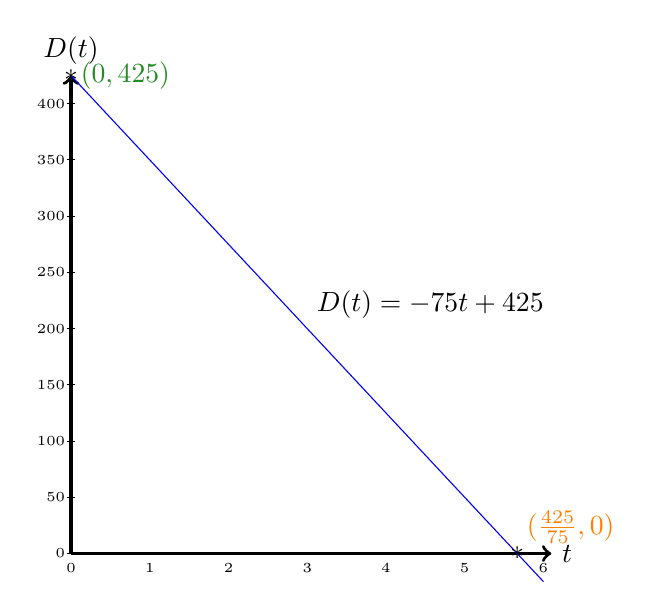
\begin{tikzpicture}[yscale=1/70]
    %\draw[gray!50, thin, step=5] (0,-20) grid (40,60);
    \draw[very thick,->] (0,0) -- (6.1,0) node[right] {$t$};
    \draw[very thick,->] (0,0) -- (0,425.1) node[above] {$D(t)$};

    \foreach \x in {0,1,...,6} \draw (\x,0.05) -- (\x,-0.05) node[below] {\tiny\x};
    \foreach \y in {0,50,...,425} \draw (-0.05,\y) -- (0.05,\y) node[left] {\tiny\y};



    \draw[scale=1,domain=0:6,smooth,variable=\x,blue] plot ({\x},{-75*\x+425});

\draw (3,200) --node[above right]{$D(t)=-75t+425$}(3,200);


\node at (0,425){$*$};
\draw[ForestGreen] (0,425) --node[right]{$(0,425)$}(0,425);

\node at (17/3,0){$*$};
\draw[orange] (17/3,0) --node[above right]{$(\frac{425}{75},0)$}(17/3,0);


\end{tikzpicture}$$  
 \url{https://www.desmos.com/calculator/dilrensiar}
    
\end{enumerate}


\end{example}


\begin{example}\label{Example:}
\Q Consider the following graphs of functions $q=S(p), D(p)$, where $p$ is the price of a product, and $q$ is the quantity demanded.

$$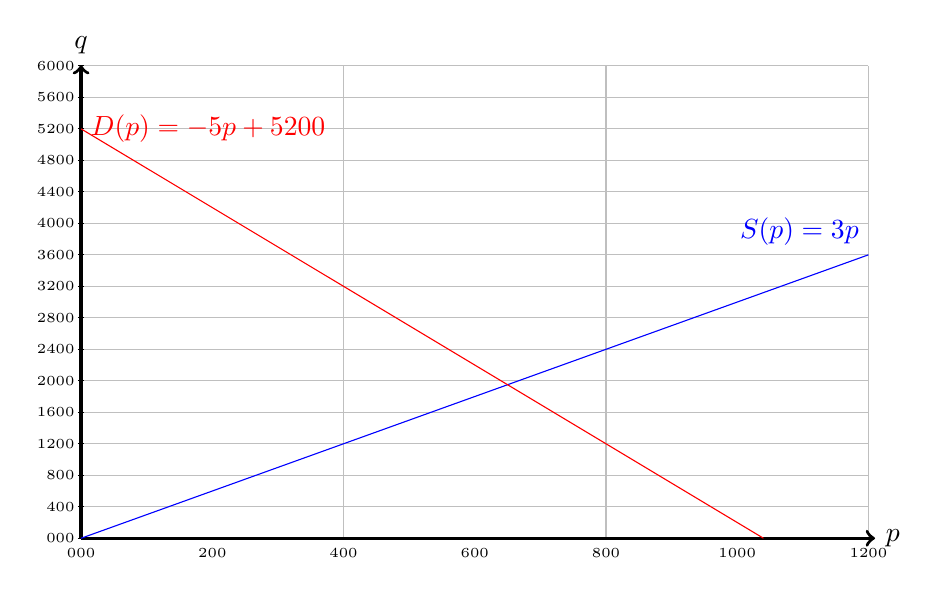
\begin{tikzpicture}[yscale=6/60, xscale=10/12]
    \draw[gray!50, thin, step=4] (0,0) grid (12,60);
    \draw[very thick,->] (0,0) -- (12.1,0) node[right] {$p$};
    \draw[very thick,->] (0,0) -- (0,60.1) node[above] {$q$};

    \foreach \x in {0,2,...,12} \draw (\x,0.05) -- (\x,-0.05) node[below] {\tiny\x00};
    \foreach \y in {0,4,...,60} \draw (-0.05,\y) -- (0.05,\y) node[left] {\tiny\y00};



    \draw[scale=1,domain=0:12,smooth,variable=\x,blue] plot ({\x},{3*\x});

    \draw[scale=1,domain=0:10.4,smooth,variable=\x,red] plot ({\x},{-5*\x+52});

\draw[red] (0,52) --node[right]{$D(p)=-5p+5200$}(0,52);
\draw[blue] (12,36) --node[above left]{$S(p)=3p$}(12,36);



\end{tikzpicture}$$

\begin{enumerate}
    \item Find the equations for the supply and demand curves $q=S(p), q=D(p)$, where $p$ is the price in dollars and $q$ is the quantity, either demanded or supplied.
    \item If \$350 is charged for this product, What is the surplus or deficit of products produced?
    \item Where is the equilibrium point (where supply and demand are the same)?
\end{enumerate}

\Sol

\begin{enumerate}
    \item It helps if we can identify some points on these lines.  We will work on them one at a time.
    \begin{enumerate}
        \item Graphically, we can see that $S(0)=0$, thus $(0,0)$ is on the supply line.  This also tells us the $q$-intercept, $b=0$.  We can also see that when $p=400, S(400)=1200$, thus $(400,1200)$ is also on this line.  Thus: $$m=\frac{1200-0}{400-0}=3.$$  So $S(p)=3p$.
        
        \item Graphically, we can see that $D(0)=5200$, thus $(0,5200)$ is on the demand line.  This also tells us the $q$-intercept, $b=5200$.  We can also see that when $p=400, D(400)=3200$, thus $(400,3200)$ is also on this line.  Thus: $$m=\frac{3200-5200}{400-0}=\frac{-2000}{400}=-5.$$  So $D(p)=-5p+5200$.
    \end{enumerate}
    \item When $p=350$, we will have $S(350)=3*350=1050$ products supplied, but $D(350)=-5*250+5200=3450$ demanded.  Thus there is a deficit of $3450-1050=2400$ products demanded that are not supplied, since demand exceeds supply.
    $$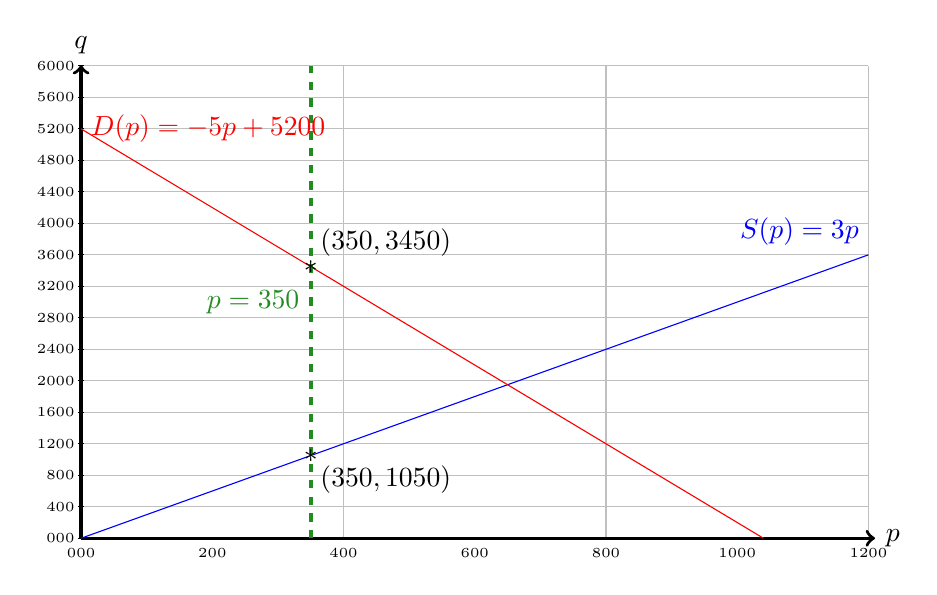
\begin{tikzpicture}[yscale=6/60, xscale=10/12]
    \draw[gray!50, thin, step=4] (0,0) grid (12,60);
    \draw[very thick,->] (0,0) -- (12.1,0) node[right] {$p$};
    \draw[very thick,->] (0,0) -- (0,60.1) node[above] {$q$};

    \foreach \x in {0,2,...,12} \draw (\x,0.05) -- (\x,-0.05) node[below] {\tiny\x00};
    \foreach \y in {0,4,...,60} \draw (-0.05,\y) -- (0.05,\y) node[left] {\tiny\y00};



    \draw[scale=1,domain=0:12,smooth,variable=\x,blue] plot ({\x},{3*\x});

    \draw[scale=1,domain=0:10.4,smooth,variable=\x,red] plot ({\x},{-5*\x+52});

    \draw[dashed, ultra thick, ForestGreen] (3.5,0) --node[left]{$p=350$} (3.5,60);

    \draw[red] (0,52) --node[right]{$D(p)=-5p+5200$}(0,52);
    \draw[blue] (12,36) --node[above left]{$S(p)=3p$}(12,36);
    
    \node at (3.5,34.5){$*$};
\draw (3.5,34.5) --node[above right]{$(350,3450)$}(3.5,34.5);

    \node at (3.5,10.5){$*$};
\draw (3.5,10.5) --node[below right]{$(350,1050)$}(3.5,10.5);


\end{tikzpicture}$$
\url{https://www.desmos.com/calculator/dee7rqh07j}

\item The equilibrium point is the point where the quantity supplied and demanded are the same.  Algebraically, this means $D(p)=S(p)$, and so:

\begin{eqnarray*}
-5p+5200&=&3p\\
5200&=&8p\\
p&=&\frac{5200}{8}=650.
\end{eqnarray*}

So the equilibrium happens when $p=650$ that is \$650 per unit.  Then, we note that $S(650)=3*650=1950$ and $D(p)=-5*650+5200=1950$, so the equilibrium point is $(650, 1950)$ or $\$650$ per unit, and 1950 units sold.

$$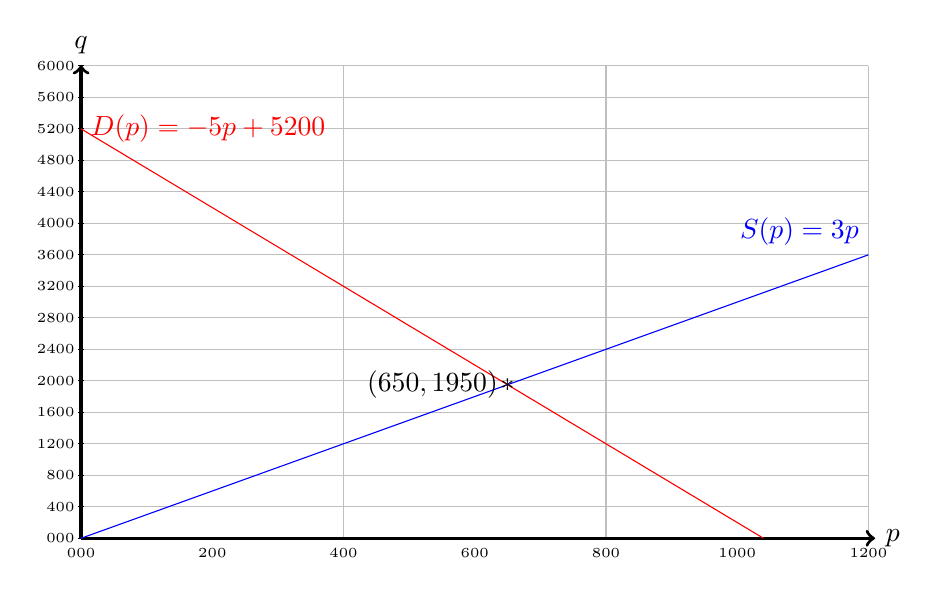
\begin{tikzpicture}[yscale=6/60, xscale=10/12]
    \draw[gray!50, thin, step=4] (0,0) grid (12,60);
    \draw[very thick,->] (0,0) -- (12.1,0) node[right] {$p$};
    \draw[very thick,->] (0,0) -- (0,60.1) node[above] {$q$};

    \foreach \x in {0,2,...,12} \draw (\x,0.05) -- (\x,-0.05) node[below] {\tiny\x00};
    \foreach \y in {0,4,...,60} \draw (-0.05,\y) -- (0.05,\y) node[left] {\tiny\y00};



    \draw[scale=1,domain=0:12,smooth,variable=\x,blue] plot ({\x},{3*\x});

    \draw[scale=1,domain=0:10.4,smooth,variable=\x,red] plot ({\x},{-5*\x+52});

\draw[red] (0,52) --node[right]{$D(p)=-5p+5200$}(0,52);
\draw[blue] (12,36) --node[above left]{$S(p)=3p$}(12,36);

    \node at (6.5,19.5){$*$};
\draw (6.5,19.5) --node[left]{$(650,1950)$}(6.5,19.5);



\end{tikzpicture}$$
\url{https://www.desmos.com/calculator/aywru3gvxu}
\end{enumerate}

\end{example}

These examples barely scratch the surface on how linear functions may be applied, but hopefully they gave you some sense on what sort of things they can be used to model, what sort of questions one can answer with them, and how to address them when the time comes.

\section{Linear Regression}


\subsection{Philosophy of Linear Regression}

It turns out that it's fairly rare to find variables in the world that are truly independent of each other.  The world is full of variables that have hidden connections and part of understanding the universe we exist in is uncovering all these connections.  This is true since the first cave person stood near a fire and realized that standing near a fire made them warmer, thus uncovering a connection between standing near fires and warmth.\\

However, since the world is an interconnected web of hidden influences, it's rare to see two variables that can be solely and completely determined by one another.  In the example of our erstwhile caveperson, it's certain that standing near fire could make you warm, but so could standing in sunlight, so could wearing more furs.  There are a lot of factors that go into determining warmth besides proximity to flames.\\

Our goal here then is to take observations and determine whether or not they are connected, and what the connection is so we could potentially use one as a predictor for the other.  But moreover, we also want to measure how strong this connection is so that we can asses how accurate these predictions might be, and what other variables may be influencing these outcomes.


\subsection{Basic Mechanics of Linear Regression}

Wee begin with an illustrative example.

\begin{example}\label{Example:BasicRegression}

\Q Consider the data set:

$$\begin{array}{c|c}
x&y\\
\hline
1&2\\
2&2\\
3&4\\
4&4\\
5&6
\end{array}$$


If we were to plot this data, it would look like:

$$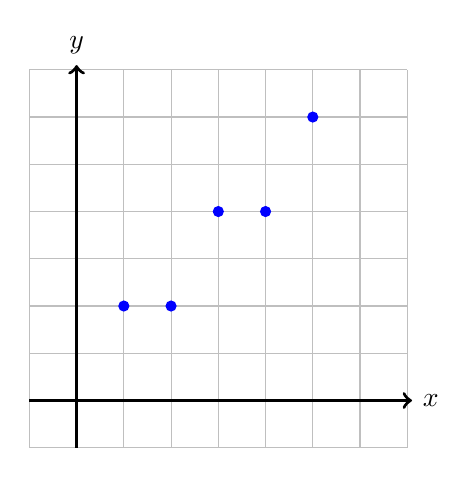
\begin{tikzpicture}[scale=.6][domain=-1:7]
    \draw[gray!50, thin, step=1] (-1,-1) grid (7,7);
    \draw[very thick,->] (-1,0) -- (7.1,0) node[right] {$x$};
    \draw[very thick,->] (0,-1) -- (0,7.1) node[above] {$y$};

%    \foreach \x in {-4,...,10} \draw (\x,0.05) -- (\x,-0.05) node[below] {\tiny\x};
%    \foreach \y in {-2,...,2} \draw (-0.05,\y) -- (0.05,\y) node[right] {\tiny\y};

\draw[blue, fill] (1,2) circle (3pt);
\draw[blue, fill] (2,2) circle (3pt);
\draw[blue, fill] (3,4) circle (3pt);
\draw[blue, fill] (4,4) circle (3pt);
\draw[blue, fill] (5,6) circle (3pt);

%  \draw[scale=1,domain=-2:2,smooth,variable=\x,blue] plot ({\x},{\x*\x*\x-3*\x}) node[above]{$y=f(x)$};


\end{tikzpicture}$$ % of mbox

Our goal here is to find a linear relationship between $x$ and $y$.  Graphically that means we want to draw a line that best fits the data we present here.  Of course, there is no line that can pass through all these points.  Our goal is to find the line that best fits these points, and to measure how well this line predicts actual values from the data.\\

\end{example}


We now commence with listing the basic arithmetic mechanics for finding a regression line.  Note that demonstrating why these formulations generate the best-fit line is beyond the scope of this text.  The most important thing to remember is: \\

``Given a bunch of points $(x_1, y_1), \ldots, (x_n, y_n)$, and a linear equation $\ell(x)=mx+b$ the \textbf{error} of each point is $e_i=\ell(x_i)-y_i$, that is the difference between the actual $y$ values, and what $\ell$ predicts should bee the $y$ values.  We are trying to find $m, b$ so that the sum of the errors squared $\sum e_i^2$ is minimized."\\

Why minimize $\sum e_i^2$?  Squaring the data erases the distinction between positive and negative error, between  over and under shoot.  Then, we want the total accumalated data to be as small as possible.




\begin{itemize}
\item $SS_X=\sum(x_i-\bar{x})^2=\sum x_i^2-\frac{(\sum x_i)^2}{n}$
\item $SS_Y=\sum(y_i-\bar{y})^2=\sum y_i^2-\frac{(\sum y_i)^2}{n}$
\item $SS_{XY}=\sum(x_i-\bar{x})(y_i-\bar{y})=\sum x_iy_i-\frac{(\sum x_i)(\sum y_i)}{n}$
\end{itemize}

The slope of the regression line will be:

$$\beta_1:=\frac{SS_{XY}}{SS_{X}}$$

If we recall, a line needs not just a slope, but a $y$ intercept.  So how can we figure out what the $y$ intercept should be?  Well, given the slope $\beta_1$, ON AVERAGE, given some $x_i$, we should get that $y_i=\beta_1x_i+\beta_0$, where $\beta_0$ is our yet-unknown $y$-intercept.  Again, this won't happen every time, or possibly ever, but it should be the average result, so the way we find $\beta_0$ is:

\begin{eqnarray*}
\bar{y}&=&\beta_1\bar{x}+\beta_0\\
\beta_0&=&\bar{y}-\beta_1\bar{x}.
\end{eqnarray*}

The above constructions are necessary to produce the best fit line.  In order to measure how good of a fit this line is, we introduce the \textbf{correlation coefficient}, usually denoted $r$.  This value is computed as follows:

$$r=\frac{n(\sum x_iy_i)-(\sum x_i)(\sum y_i)}{\sqrt{(n\sum x_i^2) - (\sum x_i)^2}\cdot \sqrt{n(\sum y_i^2)-(\sum y_i)^2}}.$$

This value measures the correction between the $x$ and $y$ values, with $r$ ranging from $-1$ to $1$.  The way we should interpret the $r$ values is as follows:

\begin{enumerate}
    \item Positive $r$ means positive correlation, meaning as $x$ goes up, $y$ tends to go up.  Negative $r$ means the opposite, as $x$ goes up, $y$ tends to go down.  Correlation of 0 means $x$'s change does not predict whether or not $y$ goes up or down.
    
    \item The closer $r$ is to 0, the weaker the correlation, meaning the ability to predict $y$ from $x$ is weak, the closer to $-1$ or $1$, the better our ability to predict $y$ from $x$.
\end{enumerate}

\begin{example}\label{Example:visualizecorr}
Consider the following plots of points.  Whether the points tend to have an upward or downward trend determines the sign of $r$, how well the best fit line predicts the points determines how close $r$ is to either $-1$ or $1$.

$$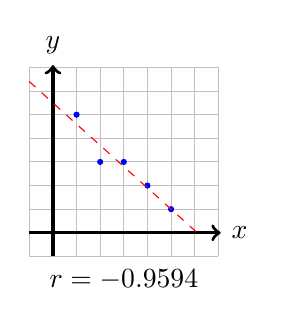
\begin{tikzpicture}[scale=.3][domain=-1:7]
    \draw[gray!50, thin, step=1] (-1,-1) grid (7,7);
    \draw[very thick,->] (-1,0) -- (7.1,0) node[right] {$x$};
    \draw[very thick,->] (0,-1) -- (0,7.1) node[above] {$y$};

%    \foreach \x in {-4,...,10} \draw (\x,0.05) -- (\x,-0.05) node[below] {\tiny\x};
%    \foreach \y in {-2,...,2} \draw (-0.05,\y) -- (0.05,\y) node[right] {\tiny\y};

\draw[blue, fill] (1,5) circle (3pt);
\draw[blue, fill] (2,3) circle (3pt);
\draw[blue, fill] (3,3) circle (3pt);
\draw[blue, fill] (4,2) circle (3pt);
\draw[blue, fill] (5,1) circle (3pt);

  \draw[scale=1,domain=-1:6.111,smooth,variable=\x,red, dashed] plot ({\x},{-0.9*\x+5.5});

\draw (3, -2) --node{$r=-0.9594$} (3,-2);

\end{tikzpicture}
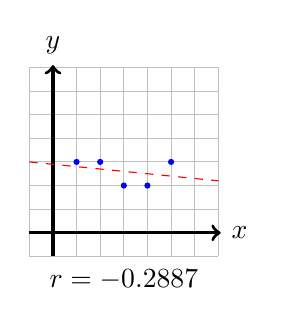
\begin{tikzpicture}[scale=.3][domain=-1:7]
    \draw[gray!50, thin, step=1] (-1,-1) grid (7,7);
    \draw[very thick,->] (-1,0) -- (7.1,0) node[right] {$x$};
    \draw[very thick,->] (0,-1) -- (0,7.1) node[above] {$y$};

%    \foreach \x in {-4,...,10} \draw (\x,0.05) -- (\x,-0.05) node[below] {\tiny\x};
%    \foreach \y in {-2,...,2} \draw (-0.05,\y) -- (0.05,\y) node[right] {\tiny\y};

\draw[blue, fill] (1,3) circle (3pt);
\draw[blue, fill] (2,3) circle (3pt);
\draw[blue, fill] (3,2) circle (3pt);
\draw[blue, fill] (4,2) circle (3pt);
\draw[blue, fill] (5,3) circle (3pt);

  \draw[scale=1,domain=-1:7,smooth,variable=\x,red, dashed] plot ({\x},{-0.1*\x+2.9});

\draw (3, -2) --node{$r=-0.2887$} (3,-2);

\end{tikzpicture}
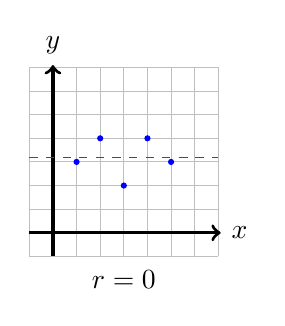
\begin{tikzpicture}[scale=.3][domain=-1:7]
    \draw[gray!50, thin, step=1] (-1,-1) grid (7,7);
    \draw[very thick,->] (-1,0) -- (7.1,0) node[right] {$x$};
    \draw[very thick,->] (0,-1) -- (0,7.1) node[above] {$y$};

%    \foreach \x in {-4,...,10} \draw (\x,0.05) -- (\x,-0.05) node[below] {\tiny\x};
%    \foreach \y in {-2,...,2} \draw (-0.05,\y) -- (0.05,\y) node[right] {\tiny\y};

\draw[blue, fill] (1,3) circle (3pt);
\draw[blue, fill] (2,4) circle (3pt);
\draw[blue, fill] (3,2) circle (3pt);
\draw[blue, fill] (4,4) circle (3pt);
\draw[blue, fill] (5,3) circle (3pt);

  \draw[scale=1,domain=-1:7,smooth,variable=\x,red, dashed] plot ({\x},{3.2});

\draw (3, -2) --node{$r=0$} (3,-2);

\end{tikzpicture}
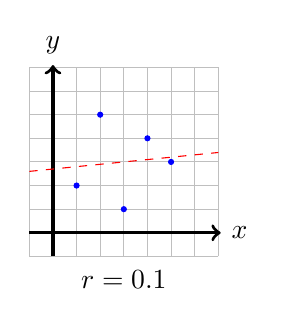
\begin{tikzpicture}[scale=.3][domain=-1:7]
    \draw[gray!50, thin, step=1] (-1,-1) grid (7,7);
    \draw[very thick,->] (-1,0) -- (7.1,0) node[right] {$x$};
    \draw[very thick,->] (0,-1) -- (0,7.1) node[above] {$y$};

%    \foreach \x in {-4,...,10} \draw (\x,0.05) -- (\x,-0.05) node[below] {\tiny\x};
%    \foreach \y in {-2,...,2} \draw (-0.05,\y) -- (0.05,\y) node[right] {\tiny\y};

\draw[blue, fill] (1,2) circle (3pt);
\draw[blue, fill] (2,5) circle (3pt);
\draw[blue, fill] (3,1) circle (3pt);
\draw[blue, fill] (4,4) circle (3pt);
\draw[blue, fill] (5,3) circle (3pt);

  \draw[scale=1,domain=-1:7,smooth,variable=\x,red, dashed] plot ({\x},{0.1*\x+2.7});

\draw (3, -2) --node{$r=0.1$} (3,-2);

\end{tikzpicture}
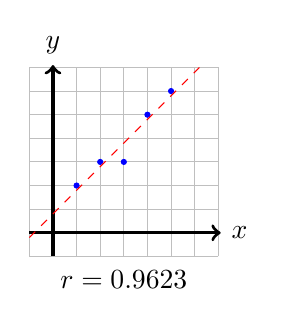
\begin{tikzpicture}[scale=.3][domain=-1:7]
    \draw[gray!50, thin, step=1] (-1,-1) grid (7,7);
    \draw[very thick,->] (-1,0) -- (7.1,0) node[right] {$x$};
    \draw[very thick,->] (0,-1) -- (0,7.1) node[above] {$y$};

%    \foreach \x in {-4,...,10} \draw (\x,0.05) -- (\x,-0.05) node[below] {\tiny\x};
%    \foreach \y in {-2,...,2} \draw (-0.05,\y) -- (0.05,\y) node[right] {\tiny\y};

\draw[blue, fill] (1,2) circle (3pt);
\draw[blue, fill] (2,3) circle (3pt);
\draw[blue, fill] (3,3) circle (3pt);
\draw[blue, fill] (4,5) circle (3pt);
\draw[blue, fill] (5,6) circle (3pt);

  \draw[scale=1,domain=-1:6.2,smooth,variable=\x,red, dashed] plot ({\x},{\x+0.8});

\draw (3, -2) --node{$r=0.9623$} (3,-2);

\end{tikzpicture}
$$
$$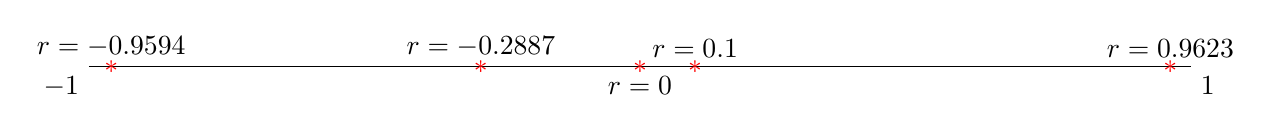
\begin{tikzpicture}[scale=7]
    \draw (-1,0)--(1,0);
    \draw (-1,0)--node[below left]{$-1$}(-1,0);
    \draw (1,0)--node[below right]{$1$}(1,0);  
    \draw[red]( 0.9623,0)--node{$*$}( 0.9623,0);
    \draw( 0.9623,0)--node[above]{$r=0.9623$}( 0.9623,0);
    \draw[red]( 0.1,0)--node{$*$}( 0.1,0);
    \draw( 0.1,0)--node[above]{$r=0.1$}( 0.1,0);
    \draw[red]( 0.0,0)--node{$*$}( 0.0,0);
    \draw( 0.0,0)--node[below]{$r=0$}( 0.0,0);
     \draw[red]( -0.2887,0)--node{$*$}( -0.2887,0);
    \draw( -0.2887,0)--node[above]{$r=-0.2887$}( -0.2887,0);
     \draw[red]( -0.9594,0)--node{$*$}( -0.9594,0);
    \draw( -0.9594,0)--node[above]{$r=-0.9594$}( -0.9594,0);
\end{tikzpicture}
$$
\end{example}

We further note that the closer $r$ is to either $-1, 1$ the closer $r^2$ is to 1, and similarly the closer $r$ is to 0, the closer $r^2$ is to 1.  Thus, we use $r^2$ as an overall measure of the strength of the correlation.  In fact, we say that $y$ is $r^2$ predicted by $x$, that is the values of $y$ are $r^2$ determinable by the values of $x$, the rest by other, as of yet undetermined variables.



\begin{example}\label{Example:BasicRegressionContd}
We continue from Example \ref{Example:BasicRegression}:

\begin{eqnarray*}
\bar{x}&=&\frac{1+2+3+4+5}{5}=3\\
\bar{y}&=&\frac{2+2+4+4+6}{5}=3.6\\
SS_X&=&(1-3)^2+(2-3)^2+(3-3)^2+(4-3)^2+(5-3)^2=10\\
SS_Y&=&(2-3.5)^2+(2-3.5)^2+(4-3.5)^2+(4-3.5)^2+(6-3.5)^2=11.25\\
SS_{XY}&=&(1-3)(2-3.5)+(2-3)(2-3.5)+(3-3)(4-3.5)+\\
&&(4-3)(4-3.5)+(5-3)(6-3.5)=10\\
\beta_1&=&\frac{10}{10}=1\\
\beta_0&=&3.6-(1)(3)=0.6
\end{eqnarray*}

So our best fit line is $y=1x+0.6$.



$$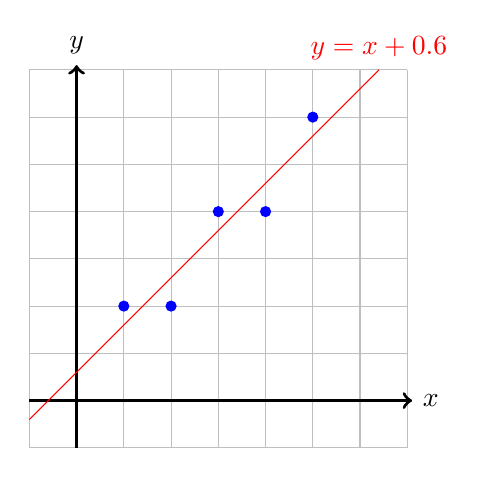
\begin{tikzpicture}[scale=.6][domain=-1:7]
    \draw[gray!50, thin, step=1] (-1,-1) grid (7,7);
    \draw[very thick,->] (-1,0) -- (7.1,0) node[right] {$x$};
    \draw[very thick,->] (0,-1) -- (0,7.1) node[above] {$y$};

%    \foreach \x in {-4,...,10} \draw (\x,0.05) -- (\x,-0.05) node[below] {\tiny\x};
%    \foreach \y in {-2,...,2} \draw (-0.05,\y) -- (0.05,\y) node[right] {\tiny\y};

\draw[blue, fill] (1,2) circle (3pt);
\draw[blue, fill] (2,2) circle (3pt);
\draw[blue, fill] (3,4) circle (3pt);
\draw[blue, fill] (4,4) circle (3pt);
\draw[blue, fill] (5,6) circle (3pt);

  \draw[scale=1,domain=-1:6.4,smooth,variable=\x,red] plot ({\x},{\x+0.6}) node[above]{$y=x+0.6$};


\end{tikzpicture}$$

Again, notice that none of the points actually fall on this line, but no possible line could have accomplished all of the points falling on it.  What we have instead is a line that passes through the points as closely as possible.  Define $e_i$ to be the error in prediction for $y_i$, that is let $e_i=y_i-(1\cdot x_i+0.6)$, then we see that:

\begin{eqnarray*}
e_1&=&2-(1+.6)=0.4\\
e_2&=&2-(2+.6)=-0.6\\
e_3&=&4-(3+.6)=0.4\\
e_4&=&4-(4+.6)=-0.6\\
e_5&=&6-(5+.6)=0.4
\end{eqnarray*}

$$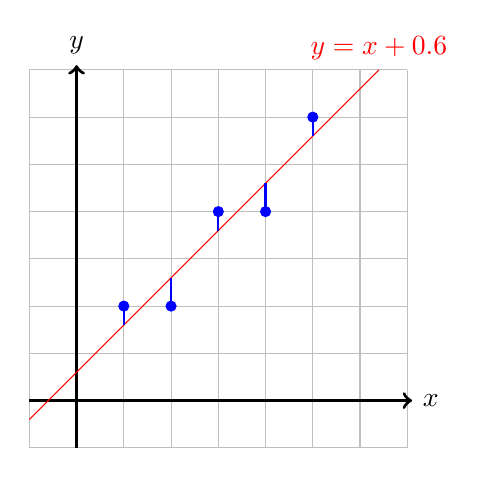
\begin{tikzpicture}[scale=.6][domain=-1:7]
    \draw[gray!50, thin, step=1] (-1,-1) grid (7,7);
    \draw[very thick,->] (-1,0) -- (7.1,0) node[right] {$x$};
    \draw[very thick,->] (0,-1) -- (0,7.1) node[above] {$y$};

%    \foreach \x in {-4,...,10} \draw (\x,0.05) -- (\x,-0.05) node[below] {\tiny\x};
%    \foreach \y in {-2,...,2} \draw (-0.05,\y) -- (0.05,\y) node[right] {\tiny\y};

\draw[blue, fill] (1,2) circle (3pt);
\draw[blue, fill] (2,2) circle (3pt);
\draw[blue, fill] (3,4) circle (3pt);
\draw[blue, fill] (4,4) circle (3pt);
\draw[blue, fill] (5,6) circle (3pt);

  \draw[scale=1,domain=-1:6.4,smooth,variable=\x,red] plot ({\x},{\x+0.6}) node[above]{$y=x+0.6$};

\draw[blue, thick](1, 1.6) -- (1,2);
\draw[blue, thick](2, 2.6) -- (2,2);
\draw[blue, thick](3, 3.6) -- (3,4);
\draw[blue, thick](4, 4.6) -- (4,4);
\draw[blue, thick](5, 5.6) -- (5,6);


\end{tikzpicture}$$


But $$e_1+e_2+e_3+e_4+e_5=(0.4)+(-0.6)+(0.4)+(0.6)+(0.4)=0.$$

This tells us this line passes through the ``middle" of the points.  Is it the best possible line?  Notice that $$\sum e_i^2=(0.4)^2+(-0.6)^2+(0.4)^2+(0.6)^2+(0.4)^2=1.2.$$  Is this the best we can do?  Again, a formal verification of this is beyond this text, but following this link: \url{https://www.desmos.com/calculator/gruczlkyyf}, you can see that by adjusting the parameters $m$ and $b$, that the sum of squares being 1.2 is the smallest error sum you can achieve.\\

To find $r$ we note that:

\begin{eqnarray*}
r&=&\frac{n(\sum x_iy_i)-(\sum x_i)(\sum y_i)}{\sqrt{(n\sum x_i^2) - (\sum x_i)^2}\cdot \sqrt{n(\sum y_i^2)-(\sum y_i)^2}}\\
&=&\frac{5(64)-(15)(18)}{\sqrt{5(55) - (15)^2}\cdot \sqrt{5(76)-(18)^2}}\\
&\approx&0.9449.
\end{eqnarray*}
So we can see that this fit is fairly close, and $x$ is a good predictor of $y$.  Since $r^2\approx 0.8929$, we can say that $y$'s value are 89.29\% determinable by $x$'s values.
\end{example}

\subsection{Good thing we don't live in the stone age.}

We should all agree that this was quite a lot of work to find these parameters for 5 values, and most data sets of work, have dozens, if not hundreds or thousands of data points.  It's simply impractical to do this by hand.\\

On the other hand a quick use of Desmos: \url{https://www.desmos.com/calculator/ir10f1wwzr} and entering the data points into the table, produces the best fit line, a plot, and the correlation coefficients.\\

Try entering your own data, adding or removing rows, and see how quickly and readily it will obtain our best fit lines and correlation coefficients!



\subsection{Applications}

\begin{example}
From fbi.gov from 2004-2013, the murder rates per 100,000 people are listed below:

$$\begin{array}{c|c}
\text{Years after 2000} & \text{Murders per 100,000 people}\\
x&y\\
\hline
4&5.5\\
5&5.6\\
6&5.8\\
7&5.7\\
8&5.4\\
9&5\\
10&4.8\\
11&4.7\\
12&4.7\\
13&4.5
\end{array}$$
\begin{enumerate}
\item Determine the best fit line for murders (per 100,000 people) $x$ years after 2000.
\item How much of a factor is the year in predictiung the number of murders?
\item Predict the murder rate in 2018.
\end{enumerate}

Entering this data in desmos: \url{https://www.desmos.com/calculator/em6xkq7udn}

\begin{enumerate}
\item It seems that the best fit line is $y=-0.144848x+6.40121$.
\item Since $r^2=0.8318$, we can say the murder rate is 83.18\% predictable by the year.
\item In 2018, the murder rate should be $-0.144848(18)+6.40121=3.793946$ or roughly 3.8 murders per 100,000 people in 2018.
\end{enumerate}




\end{example}



\begin{example}\label{Example:CorrQuizTest}
I personally wondered in quiz scores are a good predictor of test scores in Calculus.  I pulled out some data from this semester, and here are the average quiz and test scores of my students, anonymously of course:


$$\begin{array}{c|c}
\text{Quiz Average} & \text{Test Average}\\
x&y\\
\hline
87.5&100\\
76.13&94\\
75.83&93.5\\
53.53&83.5\\
76.13&83\\
71.13&78.85\\
56.13&76.5\\
73.57&70\\
66.13&69.5\\
66.13&63
\end{array}$$



\end{example}
\begin{enumerate}
\item Find the linear relationship between Quiz grades and Test grades.
\item Are Quiz grades a good predictor of Test grades?
\item If someone has an 80 average on Quizzes, predict their Test grade.
\end{enumerate}

So, once again:  \url{https://www.desmos.com/calculator/atipunytb1}

\begin{enumerate}
\item The relationship here is: $y=0.639883x+36.2168$, so there is a positive correlation, which we expect.
\item $r^2=0.2906$, so Test grades 29.06\% predictable by Quiz grades, which one would also expect, some people perform better in the Exam situation and some people perform worse.
\item We would have an expected test grade of $y=0.639883(80)+36.2168=87.40744$ or about 87.41\%.  But of course with an $r^2$ that small we shouldn't expect this to be terribly accurate.
\end{enumerate}


\subsection{Correlation $\neq$ Causation!}

A common misconception about correlated variables is that a strong correlation means that the $x$ variables \textbf{causes} the $y$ variable.  This is sometimes the case, but very often not true.\\

It is just as possible that $y$ causes $x$, or that $x$ and $y$ \textbf{share} common causes, or there's always complete coincidence.\\

In Example \ref{Example:CorrQuizTest}, if I had simply given everyone 100 on the quizzes without looking at them, and graded the exams in normal way, they likely would not have done any better.  One could argue that they would have done worse as a result.  So a positive correlation between the variables doesn't mean that one will rise simply by virtue of the other rising.\\

The bottom line is that correlations measure the strength and form of a relationship between variables, but not the nature of the relationship.










